%&<tex>
\documentclass[notheorems,xcolor=dvipsnames]{beamer}
\usetheme{Rochester}
%\usefonttheme{serif}

%\usepackage[hmargin=2.5cm, vmargin=2cm]{geometry}
\usepackage{amssymb, mathtools, yhmath, graphicx}
\usepackage{standalone}
\usepackage[most]{tcolorbox}
%\usepackage{fontspec, type1cm, titlesec, titling, fancyhdr, tabularx}
%\usepackage{unicode-math}
\usepackage{float}
\usepackage{transparent}
\usepackage[normalem]{ulem}
\usepackage{bm}
\usepackage{array}
\usepackage{csquotes}
\usetikzlibrary{arrows}
\usetikzlibrary{arrows.meta} 
\usepackage{soul}
\usepackage[normalem]{ulem}

%\usepackage{eulervm}

\usepackage{xpatch}
\usepackage{relsize}
\usepackage{scalerel}
\usepackage{stackengine}
\usepackage{gauss}
%\usepackage[abbreviations, per-mode=symbol]{siunitx}
\usepackage[CheckSingle, CJKmath]{xeCJK}
\usepackage{fontspec}
\defaultfontfeatures{Mapping=tex-text}
\usefonttheme{professionalfonts}
\usepackage{concmath}
%\usepackage{CJKulem}
%\usepackage{enumitem}
\usepackage{tikz}
\usetikzlibrary{calc, fit, backgrounds}
\usetikzlibrary{tikzmark}
\tikzset {
  overlay node/.style={
    anchor=base, outer sep=0mm, inner sep=0mm,
  }
}
\usepackage{minted}
% \usepackage{python}
% \usepackage{algorithm2e}
\definecolor{mgray}{rgb}{0.85, 0.85, 0.85}
\colorlet{mgreen}{green!70!black}
\newmintinline{cpp}{bgcolor=mgray}
\def\codesize{\fontsize{9}{12}\selectfont}
\setmonofont[Mapping=]{Source Code Pro}
%\setmonofont[Contextuals={Alternate}]{Fira Code}
\setminted{fontsize=\codesize, linenos, frame=lines, mathescape, autogobble}
%\usemintedstyle{monokai}
%\usepackage{circuitikz}
%\setCJKmainfont[BoldFont=cwTex Q Hei]{cwTex Q Ming}
%\setCJKsansfont[BoldFont=cwTex Q Hei]{cwTex Q Ming}
%\setCJKmonofont[BoldFont=cwTex Q Hei]{cwTex Q Ming}
\setCJKmainfont[AutoFakeSlant,BoldFont=Source Han Sans TW Bold]{Noto Sans CJK TC}
\newfontfamily\SHSTW{Source Han Sans TW}

\def\ofootnotesize{\fontsize{8}{12}}
\def\footnotesize{\fontsize{6}{8}\selectfont}
%\def\normalsize{\fontsize{12}{18}\selectfont}
%\def\large{\fontsize{14}{21}\selectfont}
%\def\Large{\fontsize{16}{24}\selectfont}
%\def\LARGE{\fontsize{18}{27}\selectfont}
%\def\huge{\fontsize{20}{30}\selectfont}

%\titleformat{\section}{\bf\Large}{\arabic{section}}{24pt}{}
%\titleformat{\subsection}{\large}{\arabic{subsection}.}{12pt}{}
%\titlespacing*{\subsection}{0pt}{0pt}{1.5ex}

%\usepackage{parskip}
%\parindent=24pt
%\parskip=1em

\setlength{\parskip}{\baselineskip} 
\usepackage{trimclip}
\DeclareRobustCommand\Longrightarrow{\NewRelbar\joinrel\Rightarrow}
\DeclareRobustCommand\Longleftarrow{\Leftarrow\joinrel\NewRelbar}

\makeatletter
\DeclareRobustCommand\NewRelbar{%
  \mathrel{%
    \mathpalette\@NewRelbar{}%
  }%
}
\newcommand*\@NewRelbar[2]{%
  % #1: math style
  % #2: unused
  \sbox0{$#1=$}%
  \sbox2{$#1\Rightarrow\m@th$}%
  \sbox4{$#1\Leftarrow\m@th$}%
  \clipbox{0pt 0pt \dimexpr(\wd2-.6\wd0) 0pt}{\copy2}%
  \kern-.2\wd0 %
  \clipbox{\dimexpr(\wd4-.6\wd0) 0pt 0pt 0pt}{\copy4}%
}
\makeatother



\newcommand{\img}{\mathsf{i}}
\newcommand{\ex}{\mathsf{e}}
\newcommand{\dD}{\mathrm{d}}
\newcommand{\dI}{\,\mathrm{d}}
\newcommand{\linearprog}[3][maximize]{%
\begin{array}{rl}
  \text{#1} & \kern 1em {#2} \\[8pt]
  \text{subject to} & {\renewcommand\arraystretch{1.1} #3}
\end{array}%
}

\newcommand\abs[1]{\left\lvert #1 \right\rvert}
\newcommand{\ord}{\mathcal{O}}
\newcommand{\fourier}{\mathcal{F}}
\newcommand*{\defeq}{\triangleq}
\renewcommand*{\sharp}{\mathlarger{\#}}
\newcommand*{\bZ}{\mathbb{Z}}
\newcommand*{\bF}{\mathbb{F}}
\newcommand*{\correspond}{\mathrel{\stackon[1.5pt]{=}{\stretchto{%
    \scalerel*[\widthof{=}]{\wedge}{\rule{1ex}{3ex}}}{0.5ex}}}}
\newcommand*{\Expect}{{\rm I\kern-.3em E}}
\newcommand{\btitle}[1]{{\secname} -- #1}
\newcommand{\disskip}[1][1]{\vspace*{-#1\parskip}}%
\renewcommand*{\sharp}{\mathlarger{\#}}
\newcommand{\tikzoverlay}[2]{\tikz[baseline, remember picture]{ \node[overlay node] (#1) {#2}}}%

\theoremstyle{definition}
\newtheorem{theorem}{定理}
\newtheorem{lemma}{引理}
\newtheorem{property}{性質}
\newtheorem{corollary}{推論}
\newtheorem{conjecture}{猜想}
\newtheorem{problem}{題目}

%\colorlet{origintitlefg}{block title.fg}
%\setbeamercolor{origintitle}{use=block,fg=block title.fg,bg=block title.bg}
%\setbeamercolor{originbody}{use=block body,fg=block body.fg,bg=block body.bg}

\newtheorem{definition}{定義}
\BeforeBeginEnvironment{definition}{%
  \setbeamercolor{block title}{fg=white,bg=red!70!black}
  \setbeamercolor{block body}{fg=black, bg=block title.bg!10!bg}
}
\AfterEndEnvironment{definition}{
    \setbeamercolor{block title}{use=structure,fg=white,bg=structure.fg!75!black}
    \setbeamercolor{block body}{parent=normal text,use=block title,bg=block title.bg!10!bg}
}

\newenvironment{missue}{%
\setbeamercolor{block title}{bg=ForestGreen,fg=white}
\setbeamercolor{block body}{bg=blue!20!green!20,fg=black}
\begin{block}{\centering 問題}}{\end{block}}

\newenvironment{exercise}{%
\setbeamercolor{block title}{bg=ForestGreen,fg=white}
\setbeamercolor{block body}{bg=blue!20!green!20,fg=black}
\begin{block}{習題}}{\end{block}}

\renewenvironment{proof}{%
\begin{tcolorbox}[frame empty] {\bf 證明:}\ }{\end{tcolorbox}}

%\setbeamercovered{transparent}
%\usefonttheme[onlymath]{serif}
%\settowidth{\leftmargini}{\usebeamertemplate{itemize item}}

%\makeatletter
%\patchcmd\beamer@@tmpl@frametitle{\insertframetitle}{\insertsection-\insertframetitle}{}{}
%\makeatother

\setbeamertemplate{enumerate item}{%
  \usebeamercolor[bg]{item projected}%
  \raisebox{0.28ex}{\colorbox{bg}{\color{fg}\scriptsize\insertenumlabel}}%
}

\setbeamertemplate{itemize item}{%
  \usebeamercolor[bg]{item projected}%
  \raisebox{0.25ex}{\scriptsize$\blacksquare$}%
}

\AtBeginSection[]{
  \begin{frame}
    \tableofcontents[currentsection]
  \end{frame}
  \begin{frame}
  \vfill
  \centering
  \begin{beamercolorbox}[sep=6pt,center,shadow=true,rounded=true]{title}
    \usebeamerfont{title}\LARGE\insertsectionhead\par%
  \end{beamercolorbox}
  \vfill
  \end{frame}

}

\makeatletter
\let\save@measuring@true\measuring@true
\def\measuring@true{%
  \save@measuring@true
  \def\beamer@sortzero##1{\beamer@ifnextcharospec{\beamer@sortzeroread{##1}}{}}%
  \def\beamer@sortzeroread##1<##2>{}%
  \def\beamer@finalnospec{}%
}
\makeatother

\title{基礎資料結構}
\author{yp155136}

\renewcommand*{\emph}[1]{{\bfseries #1}}

\begin{document}

\begin{frame}
  \titlepage
\end{frame}

\begin{frame}{講義勘誤}
  \begin{itemize}
    \item 第 19 頁範例 code 第 7 行「路徑壓縮」這個註解劃掉(我打錯了)
    \item 第 28 頁「實作」區第二段第三行「來找出每個數字是第幾大」中的「第幾大」改成「第幾小」
    \item 第 43 頁程式碼片段 1-14 的標題應該是「線段樹:區間加值、區間最大值」
    \item 第 60 頁習題 1-39 的題號應該是 TIOJ 1976
    \item 第 73 的程式碼片段 1-31
      \begin{itemize}
        \item 第 17, 18 行中間插入 \texttt{t->rc->fa = t;}
        \item 第 14, 15 行中間插入 \texttt{t->lc->fa = t;}
      \end{itemize}
  \end{itemize}
\end{frame}

\begin{frame}{道歉啟示}
  \begin{itemize}
    \item 範例 code 我會盡快整理好後放在 github 上的
  \end{itemize}
\end{frame}

\begin{frame}{講師簡介}
  \begin{itemize}
    \item yp155136
    \item LYB / BBCube
    \begin{itemize}
      \item ICPC 2021 台北站第二名
    \end{itemize}
    \item IOI 2018 國際資訊奧林匹亞銀牌
    \item APIO 2018 亞太資訊奧林匹亞金牌
    \only<2> {
    \item 因為想學習基礎資料結構所以當基礎資料結構講師
    }
  \end{itemize}
\end{frame}

% \begin{frame}{大綱}
%   \tableofcontents
% \end{frame}
\begin{frame}{大綱}
  \begin{itemize}
    \item 並查集
    \item 好用的 STL
    \item Sparse Table
    \item 基礎線段樹
    \item BIT
    \item 進階線段樹
    \item 樹堆
  \end{itemize}
\end{frame}

\begin{frame}{前言}
  \begin{itemize}
    \item 這堂課會教大家在競程上常用的資料結構
    \item 學會、精熟這些資料結構,可以提昇在競程上的實力喔
  \end{itemize}
\end{frame}

\documentclass[standalone]{beamer}

\begin{document}
\section{並查集}

\begin{frame}{並查集}
  \begin{itemize}
    \item 支援合併及查詢集合的資料結構
    \item 具體來說,需要支援:
    \begin{enumerate}
      \item init($n$) : 初始 $n$ 個元素,各自屬於一個獨立的集合。
      \item union($a, b$) : 將 $a$ 元素所在的集合以及 $b$ 元素所在的集合合併。
      \item find($a$) : 詢問 $a$ 所在的集合編號。
    \end{enumerate}
    \item 維護的集合兩兩互斥
    \item 來畫圖解釋吧!
  \end{itemize}
\end{frame}

\begin{frame}{\btitle{實作方法}}
  \begin{itemize}
    \item 將每個集合以樹狀結構來表示
    \item 整個並查集會形成一個森林,而每棵樹分別代表一個集合
    \item 每個元素記錄自身的父節點(程式碼中的 $p$),而每棵樹便以根節點($p[i] = i$ 的點)作爲代表
    \item 在做集合相關操作的時候,\textbf{必須要用代表點(也就是根節點)}來操作
  \end{itemize}
\end{frame}

\begin{frame}[fragile]{\btitle{範例實作}}
  \begin{minted}[breaklines]{cpp}
    struct DisjointSet {
      int p[maxn];
      void init(int n) {
        for (int i = 1; i <= n; i++)
          p[i] = i;
      }
      int find(int x) { return x == p[x] ? x : find(p[x]); }
      void join(int x, int y) { p[find(x)] = find(y); }
    };
  \end{minted}
\end{frame}

\begin{frame}{\btitle{時間複雜度}}
  \begin{itemize}
    \item \texttt{init()}:就是個 $O(N)$
    \item \texttt{find(x)}:看起來好像很快,但其實 worst case 會到 $O(N)$(樹是一條鏈的狀況)
    \item \texttt{join(x, y)}:就是個 $O(1)$
    \item 想想看,\texttt{find(x)} 真的需要 $O(N)$ 那麼多嗎?
  \end{itemize}
\end{frame}

\begin{frame}[fragile]{\btitle{範例實作}}
  \begin{itemize}
    \item \texttt{find()} 事實上就是在樹上不斷往父節點爬
    \item 把查詢路徑上所有人的父節點設爲根節點!
    \item 關心的只是每個節點屬於哪個集合,樹狀結構長什麼樣子並不重要
    \item \texttt{return x == p[x] ? x : p[x] = find(p[x]);}
    \item 經過這個改善後,複雜度\textbf{均攤}下來是 $O(N \log N)$
    \item \textbf{路徑壓縮}
  \end{itemize}
\end{frame}

\begin{frame}[fragile]{\btitle{範例實作}}
  \begin{itemize}
    \item 那 \texttt{join()} 呢?有沒有比較厲害的 join 方式可以降低複雜度?
    \item \textbf{union by rank}
    \item 維護每棵樹當前的深度
    \item 每次要合併時,都將深度小的接到深度大的上
    \item 於是,這樣樹的深度就不會超過 $O(\log n)$,\texttt{find()} 在沒有路徑壓縮下複雜度也是好的
  \end{itemize}
\end{frame}

\begin{frame}[fragile]{\btitle{範例實作}}
  \begin{minted}[breaklines]{cpp}
    void join(int x, int y) {
      x = find(x), y = find(y);
      if (x == y)
        return;
      if (rk[x] < rk[y]) // union by rank
        swap(x, y);
      p[y] = x;
      if (rk[x] == rk[y])
        ++rk[x];
    }
  \end{minted}
\end{frame}

\begin{frame}[fragile]{\btitle{實作總結}}
  \begin{itemize}
    \item 什麼都不做會退化到 $O(N)$
    \item union by rank / 路徑壓縮只用一個的話可以讓複雜度變 $O(\log N)$
    \item 同場加碼:union by rank 跟路徑壓縮一起做的話,均攤時間複雜度爲 $O( \alpha( n ) )$,幾乎可以視為 $O(1)$!
    \item 同場加碼:union by size (小樹接到大樹)跟 union by rank 的效果是一樣的喔!
  \end{itemize}
\end{frame}

\begin{frame}{\btitle{例題}}
  \begin{problem}[經典問題(這題講義上沒有)]
    給你一張 $N$ 個點的圖 $G$,圖一開始沒有任何邊,以及 $M$ 筆操作。

    操作有三種:
    \begin{itemize}
      \item 加邊:給 $a, b$,把點 $a$ 跟點 $b$ 中間加上一條邊
      \item 詢問一:給 $a, b$,問 $a, b$ 是否在同一個連通塊
      \item 詢問二:詢問目前的圖有多少個連通塊
    \end{itemize}

    \begin{itemize}
      \item $N, M \leq 10^5$
    \end{itemize}
  \end{problem}
\end{frame}

\begin{frame}{並查集}
  \begin{itemize}
    \item 並查集很常用的地方:維護圖的連通性
    \item 並查集的集合\textbf{維護連通塊}
    \item 一開始圖是空的,相當於所有點都在自己的連通塊裡面,對應到\texttt{init(N)}!
    \item 有一條邊新增進來的時候,相當於把兩個連通塊變成一個連通塊
    \item 也相當於是並查集的 \texttt{join()} 操作!
  \end{itemize}
\end{frame}

\begin{frame}{並查集}
  \begin{itemize}
    \item 詢問兩點是否連通?
    \item 判斷兩個點是不是在同一個集合
    \item \texttt{djs.find(a) == djs.find(b)}
    \item 詢問連通塊個數?
    \item 一邊 \texttt{join()} 一邊維護
    \item 每當 \texttt{join()} 兩個不同的集合時,連通塊個數\texttt{ -= 1}。
  \end{itemize}
\end{frame}

\begin{frame}{\btitle{例題}}
  \begin{problem}[Ural 1671 Anansis Cobweb]
    給一張無向圖 $G$,$N$ 個點、$M$ 條邊。
    $Q$ 筆操作,每筆操作破壞一條邊後問連通塊個數。

    \begin{itemize}
        \item
            $1 \leq N \leq 10^5$
        \item
            $1 \leq M \leq 10^5$
        \item
            $1 \leq Q \leq M$
    \end{itemize}
  \end{problem}
\end{frame}

\begin{frame}{並查集}
  \begin{itemize}
    \item 但,這題是破壞邊,不是增加邊,怎麼辦?
  \end{itemize}
\end{frame}

\begin{frame}{並查集}
  \begin{itemize}
    \item \textbf{時間倒流}
    \item 沒有被破壞的邊表示從頭到尾都沒被破壞,可以在此刻維護一個並查集
    \item 破壞一條邊,就相當於建造一條邊!
  \end{itemize}
\end{frame}

\begin{frame}{\btitle{例題}}
  \begin{problem}[POJ 1182 食物鏈]
    有三類動物 $A, B, C$,這三類動物的食物鏈構成如下:$A$ 吃 $B$, $B$ 吃 $C$,$C$ 吃 $A$。 
    現有 $N$ 個動物,編號 $1, 2, \ldots, N$。
    每個動物都是 $A,B,C$ 中的一種,但並不知道是哪一種。 
    依序給 $K$ 條屬於以下兩種的敘述:
    \begin{itemize}
      \item \texttt{1 X Y},表示 $X$ 和 $Y$ 是同類
      \item \texttt{2 X Y},表示 $X$ 吃 $Y$
    \end{itemize}
    然而,並不是每條描述都是正確的,有些是真話,有些是假話。
    
    如果當前的話與前面的某些真話衝突,就是假話
    
    請判斷哪些話是真話,哪些話是假話。
  \end{problem}
\end{frame}

\begin{frame}{並查集}
  \begin{itemize}
    \item 並查集的經典變化!
    \item 第一種資訊,顯然可以用並查集維護
    \item 假設 $a, b$ 同類,可能可以類似 \texttt{djs.join(a, b)}
    \item 但,第二種資訊怎麼辦?好像沒辦法直接維護ㄋㄟ
  \end{itemize}
\end{frame}

\begin{frame}{並查集}
  \begin{itemize}
    \item 那就直接假設每種動物在每個分類底下的狀況!
    \item 把每個動物 $i$ 分成三個資訊:動物 $i$ 屬於第 $A$ 類、動物 $i$ 屬於第 $B$ 類、動物 $i$ 屬於第 $C$ 類
    \item 假設 $i_O$ 代表動物 $i$ 是第 $O$ 類的資訊
    \item 有了這個可以做什麼 OuO
  \end{itemize}
\end{frame}

\begin{frame}{並查集}
  \begin{itemize}
    \item 我們可以用並查集維護\textbf{資訊間的因果關係}
    \item 一個集合裡面的資訊代表「這些資訊必須同時發生」
    \item 比如說,假設 $(x, y)$ 符合第一種資訊
    \item 那就代表:如果 $x$ 是 $A$ 類,那 $y$ 必須是 $A$ 類,反之亦然($B, C$ 類同樣可以套用)
    \item 翻譯一下:如果 $x_A$ 發生的話,那 $y_A$ 也一定要發生($B, C$ 類同樣可以套用)
    \item $join(x_A, y_A), join(x_B, y_B), join(x_C, y_C)$
  \end{itemize}
\end{frame}

\begin{frame}{並查集}
  \begin{itemize}
    \item 我們可以用並查集維護\textbf{資訊間的因果關係}
    \item 一個集合裡面的資訊代表「這些資訊必須同時發生」
    \item 比如說,假設 $(x, y)$ 符合第二種資訊
    \item 那就代表:
    \begin{itemize}
      \item 如果 $x$ 是 $A$ 類,那 $y$ 必須是 $B$ 類,反之亦然
      \item 如果 $x$ 是 $B$ 類,那 $y$ 必須是 $C$ 類,反之亦然
      \item 如果 $x$ 是 $C$ 類,那 $y$ 必須是 $A$ 類,反之亦然
    \end{itemize}
    \item $join(x_A, y_B), join(x_B, y_C), join(x_C, y_A)$
  \end{itemize}
\end{frame}

\begin{frame}{並查集}
  \begin{itemize}
    \item 我們可以用並查集維護\textbf{資訊間的因果關係}
    \item 一個集合裡面的資訊代表「這些資訊必須同時發生」
    \item 判斷真假?
    \item 一種判斷方法:如果 join 後發生 $find(x_A) == find(x_B)$,就代表這中間一定有假話!
  \end{itemize}
\end{frame}

\begin{frame}{\btitle{例題}}
  \begin{problem}[經典問題]
    給一張無向圖 $G$,$N$ 個點、$M$ 條邊。
    
    (版本一)請你判斷這張圖是不是二分圖?

    (版本二)請你判斷這張圖存不存在長度是奇數的簡單環?
  \end{problem}

  這題是上個例題的簡化版,也是一個並查集非常實用的地方ㄛ!
\end{frame}

\begin{frame}{\btitle{總結}}
  \begin{itemize}
    \item 並查集是一個維護集合的工具
    \item 常用在圖論上維護圖的連通性
    \item 有蠻酷的變形
    \item 有時候會跟時間線段樹搭配,歡迎參考進階資料結構的講義!
  \end{itemize}
\end{frame}

\end{document}


\documentclass[standalone]{beamer}

\begin{document}
\section{好用的 STL}

\begin{frame}{好用的 STL}
  \begin{itemize}
    \item STL 裡面有許多實用的東西
    \item 這個章節會選一些介紹,剩下的就麻煩大家自行上網搜尋ㄛ
  \end{itemize}
\end{frame}

\begin{frame}{\btitle{bitset 例題}}
  \begin{problem}[NEOJ 743 數字總和]
    給你 $N$ 個數字 $a_1, a_2, \dots, a_N$,並且滿足 $\sum_{i = 1}^{N} a_i \le M$。

    現在,對於每個數字 $x$ ,請判斷 $x$ 可不可由 $a_1, a_2, \dots, a_N$ 給湊出來。也就是說,能不能找到一個集合 $S$ ,使得 $\sum_{i \in S} a_i = x$。

    \begin{itemize}
        \item $N \leq 2 \times 10^5$
        \item $M \leq 2 \times 10^5$
    \end{itemize}
  \end{problem}
\end{frame}

\begin{frame}[fragile]{\btitle{bitset}}
  \begin{itemize}
    \item 我會 DP!
    \item
    \begin{minted}[breaklines]{cpp}
      dp[0] = 1;
      for (int i = 1; i <= n; ++i) {
        std::cin >> a[i];
        for (int x = m; x >= a[i]; --x) {
          dp[x] |= dp[x - a[i]];
        }
      }
    \end{minted}
    \item 複雜度是 $O(NM)$,TLE
    \item bitset 該出場了! 
  \end{itemize}
\end{frame}

\begin{frame}{\btitle{bitset}}
  \begin{itemize}
    \item 可以想像成一個大 bool 陣列
    \item 可以直接對這個 bool 陣列做位元操作(and, or, 左移等等)
    \begin{itemize}
      \item 做這些操作的複雜度是 $O(\frac{N}{w})$!
      \item $w$ 通常不是 $32$ 就是 $64$ ,後面會解釋!
    \end{itemize}
    \item 可是等等,上面那個轉移式可以被寫成兩個 bool 陣列做位元操作的形式嗎?
  \end{itemize}
\end{frame}

\begin{frame}[fragile]{\btitle{範例實作}}
  \begin{itemize}
    \item
    \begin{minted}[breaklines]{cpp}
      bool dp_tmp[kN] = {false};
      for (int x = a[i]; x <= m; ++x) { // step 1
        dp_tmp[x] = dp[x - a[i]];
      }
      for (int x = 0; x <= m; ++ x) { // step 2
        dp[x] = dp[x] | dp_tmp[x];
      }
    \end{minted}
    \item step 1 其實就是把 $dp$ 整個陣列往右移 $a[i]$ 格
    \item step 2 其實就是 $dp$ 跟 $dp\_tmp$ 做 and 操作
  \end{itemize}
\end{frame}

\begin{frame}[fragile]{\btitle{範例實作}}
  \begin{minted}[breaklines]{cpp}
    std::bitset<kN> dp; // 宣告一個大小為 kN 的 bitset
    dp[0] = 1; // dp[0] 可以直接存取 bitset 的第 0 個 bit,也可以直接寫值
    for (int i = 1; i <= n; ++i) {
      std::cin >> a[i];
      dp |= (dp << a[i]); // dp = dp | (dp << a[i]);
    }
  \end{minted}
\end{frame}

\begin{frame}{\btitle{bitset}}
  \begin{itemize}
    \item 複雜度瞬間變成 $O(\frac{NM}{w})$,AC
    \item $w$ 要看跑程式機器的 word 大小,通常不是 $32$ 就是 $64$
    \item 官解複雜度有除 32 或 64 通常代表有用到 bitset
    \item bitset 的更多用法歡迎參考講義喔!
  \end{itemize}
\end{frame}

\begin{frame}{\btitle{離散化}}
  \begin{itemize}
    \item 詳細的定義可以參考講義
    \item 白話文:把數字重新從 $1$ 開始按照大小填
    \item $[5, -6, 3, 5, 7]$ 變成 $[3, 1, 2, 3, 4]$
    \item 通常離散化後的數字都會是整數
    \item 常見用途:把 $[1, 10^9]$ 的數字變成 $[1, N]$ 後,就可以開一個大小是 $O(N)$ 的陣列做事
  \end{itemize}
\end{frame}

\begin{frame}[fragile]{\btitle{idea 1}}
  \begin{itemize}
    \item 把那 $N$ 個數字丟進 \texttt{std::map} 裡面
    \item 再依序把數字在 map 中對應到的 value 依序填上 $[1, N]$
    \item 最後利用 map 把原本的數字替換成新的數字
    \begin{minted}[breaklines]{cpp}
      std::map<int, int> mp;
      for (int i : a) mp[i] = 0;
      int idx = 0;
      for (auto p : mp) mp[p.first] = ++idx;
      for (int &i : a) i = mp[i];
    \end{minted}
    \item \texttt{std::map} 常數太大了,實作上並不是一個有效率的作法
  \end{itemize}
\end{frame}

\begin{frame}[fragile]{\btitle{idea 1}}
  \begin{itemize}
    \item 把所有數字由小到大排序好
    \item 利用二分搜尋法,來找出每個數字是第幾小
    \item 比如說,$[5, -6, 3, 5, 7]$ 的 $5$ 是第三小,就把 $5$ 對應到 $3$
  \end{itemize}
\end{frame}

\begin{frame}[fragile]{\btitle{範例實作}}
  \begin{minted}[breaklines]{cpp}
    std::vector<int> v;
    for (int i = 1; i <= n; ++i) {
      v.emplace_back(arr[i]);
    }
    std::sort(v.begin(), v.end());
    for (int i = 1; i <= n; ++i) {
      arr[i] = std::lower_bound(v.begin(), v.end(), arr[i]) - v.begin() + 1;
    }
  \end{minted}
  
  \texttt{std::sort} 可以用 $O(N \log N)$ 的時間來排序那 $N$ 個數字

  \texttt{std::lower\_bound} 可以在 $O(\log N)$ 的時間內找出第一個不小於目標數字的位置
\end{frame}

\begin{frame}[fragile]{\btitle{範例實作}}
  \begin{itemize}
    \item 
    \begin{minted}[breaklines]{cpp}
      std::vector<int> v;
      for (int i = 1; i <= n; ++i) {
        v.emplace_back(arr[i]);
      }
      std::sort(v.begin(), v.end());
      v.resize(std::unique(v.begin(), v.end()) - v.begin());
      for (int i = 1; i <= n; ++i) {
        arr[i] = std::lower_bound(v.begin(), v.end(), arr[i]) - v.begin() + 1;
      }
    \end{minted}

    \item \texttt{std::unique} 會把所有不同的元素搬到容器的前面,並且回傳最後一個不同元素後面的位置
    \item 拿這個回傳值跟容器的開頭相減,就可以得到總共有多少相異的元素(resize 那行在做的事情)
  \end{itemize}
\end{frame}

\begin{frame}{\btitle{離散化}}
  \begin{itemize}
    \item \texttt{std::sort} 可以用 $O(N \log N)$ 的時間來排序那 $N$ 個數字
    \item \texttt{std::lower\_bound} 可以在 $O(\log N)$ 的時間內找出第一個不小於目標數字的位置
    \item \texttt{std::unique} 會把所有不同的元素搬到容器的前面,並且回傳最後一個不同元素後面的位置,複雜度為 $O(N)$
  \end{itemize}
\end{frame}

\begin{frame}{\btitle{pbds}}
  \begin{itemize}
    \item 平板電視、黑魔法
    \item 有現成的 hash table、heap、平衡樹
    \item 平衡樹比 \texttt{std::set} 還強大,可以支援搜尋一個數字的 order (大小)
    \item 但其實不會 pbds 對競程影響不會那麼大(?)
    \item 有興趣請參考講義 + 網路資料!
  \end{itemize}
\end{frame}

\begin{frame}{\btitle{rope}}
  \begin{itemize}
    \item 簡化版持久化線段樹
    \item 有興趣請參考講義 + 網路資料!
  \end{itemize}
\end{frame}

\end{document}





\documentclass[standalone]{beamer}

\begin{document}
\section{Sparse Table}

\begin{frame}{Sparse Table}
  \begin{itemize}
    \item \(\langle {O}(f(N)), {O}(g(N))\rangle\) 來代表某個資料結構需要 \({O}(f(N))\) 預處理,並可以 \({O}(g(N))\) 回答某一個詢問
    \item 他是一個 \(\langle {O}(N \log N), {O}(1)\rangle\) 處理靜態區間最大值的資料結構
    \item 好抽象,先來看例題!
  \end{itemize}
\end{frame}

\begin{frame}{\btitle{例題}}
  \begin{problem}[區間最大值 Range Maximum Query,RMQ]
    給定一個長度為 \(N\) 的正整數序列 \(a_1, \dots, a_N\),接著有 \(Q\) 個詢問,每個詢問形如
    \begin{itemize}
        \item
            \(\texttt{1 l r}\),請你回答在 \(a_l, a_{l+1}, \dots, a_{r}\) 當中的最大值。
    \end{itemize}
    
    \begin{itemize}
        \item
            \(N, Q \leq 5 \times 10^5\)
    \end{itemize}
  \end{problem}

  靜態:序列的數值不會變動。相對應的「動態區間最大值」會在下一個章節講喔!
\end{frame}

\begin{frame}[fragile]{\btitle{例題}}
  \begin{itemize}
    \item 我會!
    \item 
    \begin{minted}[breaklines]{cpp}
      int ret = 0;
      for (int i = l; i <= r; ++i) ret = max(ret, a[i]);
      cout << ret << '\n';
    \end{minted}
    \item 試著用 \(\langle {O}(f(N)), {O}(g(N))\rangle\) 來表達看看上面演算法的複雜度
  \end{itemize}
\end{frame}

\begin{frame}[fragile]{\btitle{例題}}
  \begin{itemize}
    \item 我會!
    \item 
    \begin{minted}[breaklines]{cpp}
      int ret = 0;
      for (int i = l; i <= r; ++i) ret = max(ret, a[i]);
      cout << ret << '\n';
    \end{minted}
    \item \(\langle {O}(1), {O}(N)\rangle\), TLE!
  \end{itemize}
\end{frame}

\begin{frame}[fragile]{\btitle{例題}}
  \begin{itemize}
    \item 我會!
    \item 
    \begin{minted}[breaklines]{cpp}
      int ans[kN][kN];
      for (int i = 1; i <= n; ++i) {
        ans[i][i] = a[i];
        for (int j = i + 1; j <= n; ++j) ans[i][j] = max(ans[i][j - 1], a[j]);
      }
      cout << ans[l][r] << '\n';
    \end{minted}
    \item 試著用 \(\langle {O}(f(N)), {O}(g(N))\rangle\) 來表達看看上面演算法的複雜度
  \end{itemize}
\end{frame}

\begin{frame}[fragile]{\btitle{例題}}
  \begin{itemize}
    \item 我會!
    \item 
    \begin{minted}[breaklines]{cpp}
      int ans[kN][kN];
      for (int i = 1; i <= n; ++i) {
        ans[i][i] = a[i];
        for (int j = i + 1; j <= n; ++j) ans[i][j] = max(ans[i][j - 1], a[j]);
      }
      cout << ans[l][r] << '\n';
    \end{minted}
    \item \(\langle {O}(N^2), {O}(1)\rangle\), TLE!
  \end{itemize}
\end{frame}

\begin{frame}[fragile]{\btitle{例題}}
  \begin{itemize}
    \item 兩種方法各有利弊:
    \begin{itemize}
      \item 第一個方法的好處是預處理超快,壞處是詢問慢到哭
      \item 第二個方法的好處是詢問超快,壞處是預處理慢到哭
    \end{itemize}
    \item 有沒有辦法在預處理跟詢問達到平衡呢?
    \item 可以!這就是 Sparse Table 厲害的地方
  \end{itemize}
\end{frame}

\begin{frame}[fragile]{Sparse Table}
  \begin{itemize}
    \item Sparse Table 希望在用相對少的預處理,來達到盡量快的詢問
    \item 暴雷一:詢問可以 $O(1)$
    \item 暴雷二:預處理是處理連續區間的最大值
    \item 既然是 $O(1)$ 回答詢問,就代表 $[ql, qr]$ 的答案需要用 $O(1)$ 個預處理資料回答
    \item 如果只用一個預處理資料的話,會變成上面 \(\langle {O}(N^2), {O}(1)\rangle\)
    \item 那如果用兩個呢?
  \end{itemize}
\end{frame}

\begin{frame}[fragile]{Sparse Table}
  \begin{itemize}
    \item 想法一:用 $[ql, mid]$ 跟 $[mid + 1, qr]$ 組出答案
    \item $mid = (ql + qr) / 1$,也就是切一半的意思
    \item 可是這樣還是要預處理長度為 $1$ 到 $\frac{N}{2}$ 的連續子序列的答案,複雜度還是 $O(N^2)$
    \item 怎麼辦?
    \item 靈光一閃!
  \end{itemize}
\end{frame}

\begin{frame}{Sparse Table}
  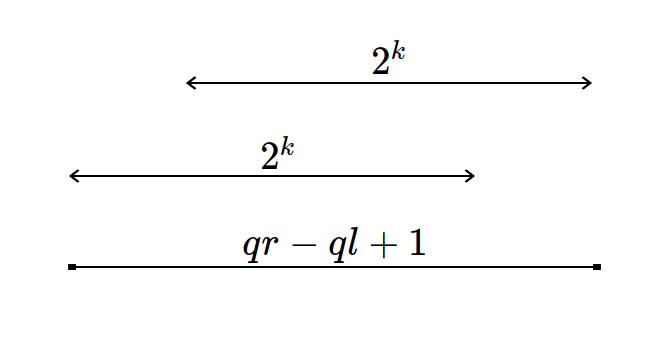
\includegraphics[width=5cm]{figures/sparse-table.png}
  \begin{itemize}
    \item 回答一個詢問 \([ql, qr]\) 最大值時,我們可以找到最大的 \(k\) 使得 \(2^k \leq qr - ql + 1\)
    \item 那麼 \([ql, qr]\) 正好可以用兩個長度 \(2^k\) 的區間的聯集湊出來!
    \item 也就是說,把序列每個位置做為開頭,長度是 $1, 2, 4, 8$ 等等 $2$ 的冪次長度的子序列的最大值存起來,就可以在 $O(1)$ 的時間回答一個詢問了
  \end{itemize}
\end{frame}

\begin{frame}{Sparse Table}
  \begin{itemize}
    \item 把序列每個位置做為開頭,長度是 $1, 2, 4, 8$ 等等 $2$ 的冪次長度的子序列的最大值存起來
    \item 看起來我們預處理的資訊有 $O(N) \times O(\log N) = O(N \log N)$ 個
    \item 令 \(f(i, j)\) 表示區間 \([i, i+2^j)\) 的最大值
    \item 也就是說,$f(i, j)$ 是從 $i$ 開始往後 $2^j$ 這個連續序列的最大值
  \end{itemize}
\end{frame}

\begin{frame}{Sparse Table}
  \begin{itemize}
    \item 把序列每個位置做為開頭,長度是 $1, 2, 4, 8$ 等等 $2$ 的冪次長度的子序列的最大值存起來
    \item 看起來我們預處理的資訊有 $O(N) \times O(\log N) = O(N \log N)$ 個
    \item 令 \(f(i, j)\) 表示區間 \([i, i+2^j)\) 的最大值
    \item 也就是說,$f(i, j)$ 是從 $i$ 開始往後 $2^j$ 這個連續序列的最大值
    \item 要怎麼更新呢?
  \end{itemize}
\end{frame}

\begin{frame}[fragile]{Spare Table}
  \begin{itemize}
    \item 
    \begin{minted}[breaklines]{cpp}
      int f[kN][klogN];
      for (int i = 0; i < kN; ++i) {
        for (int j = 0; j < klogN; ++j) {
          f[i][j] = a[i];
          for (int k = i; k < min(i + (1 << j), n); ++k) {
            f[i][j] = max(f[i][j], a[k]);
          }
        }
      }
    \end{minted}
    \item 每個預處理資料都用 $O(N)$ 算答案,複雜度為 $O(N^2 \log N)$,TLE
    \item 有辦法\textbf{重複利用已經預處理好的資料}嗎?
  \end{itemize}
\end{frame}

\begin{frame}[fragile]{Sparse Table}
  \begin{itemize}
    \item 來試試看吧!
    \item 令 \(f(i, j)\) 表示區間 \([i, i+2^j)\) 的最大值
    \item $j = 0$ 好像沒啥辦法,就是個 $f(i, 0) = a_i$
    \item $j = 1$ 呢?好像就是 $f(i, 1) = \max(a_i, a_{i + 1})$,還看不太出來
    \item $j = 2$ 呢? $f(i, 2) = \max(\{a_i, a_{i + 1}, a_{i + 2}, a_{i + 3}\})$
    \item 試著對半切切看呢?$f(i, 2) = \max(\max(a_i, a_{i + 1}), \max(a_{i + 2, i + 3}))$
    \item 咦,$\max(a_i, a_{i + 1})$ 好像是 $f(i, 1)$ 耶,$\max(a_{i + 2}, a_{i + 3})$ 好像是 $f(i + 2, 1)$
    \item 長度是 $4$ 可以被拆成 $2 + 2$!
  \end{itemize}
\end{frame}

\begin{frame}[fragile]{Sparse Table}
  \begin{itemize}
    \item 令 \(f(i, j)\) 表示區間 \([i, i+2^j)\) 的最大值
    \item 所以其實,$j = 1$ 的 $f(i, 1) = \max(a_i, a_{i + 1})$ 也可以寫成 $f(i, 1) = \max(f(i, 0), f(i + 1, 0))$
    \item 所以,假設我們已經有所有長度是 $1$ 的答案了(就是 $a$ 序列本身)
    \item 我們就會有長度是 $2$ 的答案(每個長度是 $2$ 的答案都可以由 $1 + 1$ 組出來)
    \item 我們就會有長度是 $4$ 的答案(每個長度是 $4$ 的答案都可以由 $2 + 2$ 組出來)
  \end{itemize}
\end{frame}

\begin{frame}{Sparse Table}
  \begin{itemize}
    \item 令 \(f(i, j)\) 表示區間 \([i, i+2^j)\) 的最大值
    \item 所以,比較大方向的來說,長度是 $2^j$ 的區間可以由兩個長度對半($2^{j - 1}$)區間的答案湊出來
    \item 第一段的開頭是 $i$,第二段的開頭是 $i + 2^{j - 1}$
    \item $f(i, j) = \max(f(i, j - 1), f(i + 2^{j - 1}, j - 1))$
    \item 這個更新的式子是 $O(1)$ 的!也就是說,更新一個預處理資料為 $O(1)$
    \item 預處理的複雜度為 $O(N \log N) \times O(1) = O(N \log N)$
    \item \(\langle {O}(N \log N), {O}(1)\rangle\)
  \end{itemize}
\end{frame}

\begin{frame}[fragile]{\btitle{範例實作}}
  \begin{minted}[breaklines]{cpp}
    for (int i = 0; i < n; i++)
      mx[0][i] = arr[i];
    for (int lg = 0; lg + 1 < maxlg; lg++) {
      int len = 1 << lg;
      for (int i = 0; i + len < n; i++) // 注意 i + len 不要超出邊界
        mx[lg + 1][i] = std::max(mx[lg][i], mx[lg][i + len]);
    }
  \end{minted}
\end{frame}

\begin{frame}[fragile]{\btitle{範例實作}}
  \begin{minted}[breaklines]{cpp}
    int query(int l, int r) { // returns max([l, r])
      int lg = std::__lg(r - l + 1);
      int len = 1 << lg;
      return std::max(mx[lg][l], mx[lg][r - 1 - len]);
    }
  \end{minted}

  \texttt{std::\_\_lg()} 這個函數會回傳該數字以 $2$ 為底的對數的整數部份,速度比正常的 \texttt{log2()} 快上許多
\end{frame}

\begin{frame}[fragile]{\btitle{總結}}
  \begin{itemize}
    \item $O(N \log N)$ 預處理,$O(1)$ 查詢
    \item \textbf{不能支援修改}
    \item 可以用在\textbf{重複取不會對答案造成影響的詢問},比如說 gcd、bitwise-and/or
    \item 詢問很多的話可以派上用場!
    \item 思考:為什麼要用 $2^n$ 劃分,用 $3^n$ 不好嗎?
  \end{itemize}
\end{frame}

\end{document}



\documentclass[standalone]{beamer}

\begin{document}
\section{基礎線段樹}

\begin{frame}{\btitle{例題}}
  \begin{problem}[區間最大值 Range Maximum Query,RMQ]
    給定一個長度為 \(N\) 的正整數序列 \(a_1, \dots, a_N\),接著有 \(Q\) 個詢問,每個詢問形如
    \begin{itemize}
        \item
            \(\texttt{1 l r}\),請你回答在 \(a_l, a_{l+1}, \dots, a_{r}\) 當中的最大值。
        \item
            \(\texttt{2 p x}\),請你把 \(a_p\) 修改為 \(x\)。
    \end{itemize}
    
    \begin{itemize}
        \item
            \(N, Q \leq 5 \times 10^5\)
    \end{itemize}
  \end{problem}
\end{frame}

\begin{frame}{\btitle{例題}}
  \begin{itemize}
    \item 從前面的經驗來看,我們好像要對序列做一些事情,才能解決這題
    \item 前面介紹的 Sparse Table 已經派不上用場了
    \begin{itemize}
      \item 因為修改一個元素會動到將近 $O(N)$ 個預處理表格的內容 
    \end{itemize}
    \item 但 Sparse Table 的精神可以給我們一些啟發:
    \begin{itemize}
      \item 答案是從某些預處理資料組合出來的
      \item 預處理資料盡量可以由本身小資料算出大資料的答案
      \item 大資料底下的小資料大小大概都是大資料的一半
    \end{itemize}
    \item 除了 Sparse Table 精神外,我們還要支援:
    \begin{itemize}
      \item 修改一個元素的時候,讓包含這個元素的資料盡量少
    \end{itemize}
  \end{itemize}
\end{frame}

\begin{frame}{\btitle{例題}}
  \begin{itemize}
    \item \textbf{大資料底下的小資料大小大概都是大資料的一半}
    \item 不妨試試看分治吧!來看一個長度為 $5$ 的序列的分治過程
      \begin{figure}
        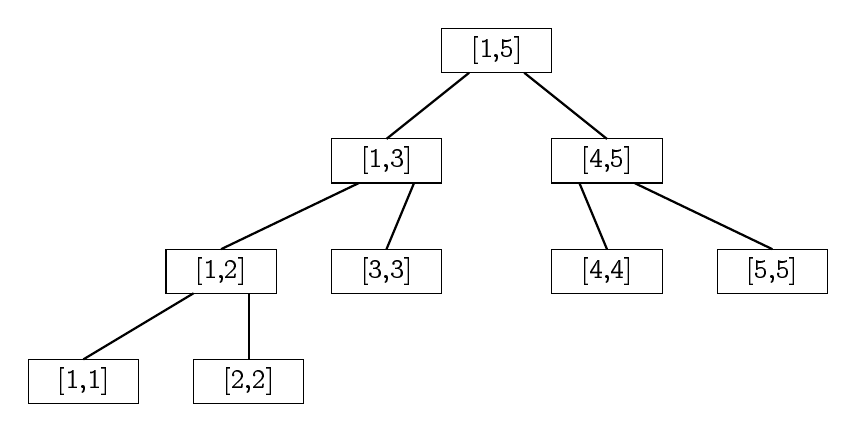
\begin{tikzpicture}[scale=0.7]
          \draw [black] (-1,7.9) rectangle (1,7.1) node [black, midway] {[1,5]}; % Draws a rectangle

          \draw [black] (-3,5.9) rectangle (-1,5.1) node [black,midway] {[1,3]}; % Draws a rectangle
          \draw [black] (1,5.9) rectangle (3,5.1) node [black,midway] {[4,5]}; % Draws a rectangle

          \draw [black] (-6,3.9) rectangle (-4,3.1) node [black,midway] {[1,2]}; % Draws a rectangle
          \draw [black] (-3,3.9) rectangle (-1,3.1) node [black,midway] {[3,3]}; % Draws a rectangle
          \draw [black] (1,3.9) rectangle (3,3.1) node [black,midway] {[4,4]}; % Draws a rectangle
          \draw [black] (4,3.9) rectangle (6,3.1) node [black,midway] {[5,5]}; % Draws a rectangle

          \draw [black] (-8.5,1.9) rectangle (-6.5,1.1) node [black,midway] {[1,1]}; % Draws a rectangle
          \draw [black] (-5.5,1.9) rectangle (-3.5,1.1) node [black,midway] {[2,2]}; % Draws a rectangle

          \draw [thick] (-0.5,7.1) to (-2,5.9);
          \draw [thick] (0.5,7.1) to (2,5.9);

          \draw [thick] (-2.5,5.1) to (-5,3.9);
          \draw [thick] (-1.5,5.1) to (-2,3.9);

          \draw [thick] (1.5,5.1) to (2,3.9);
          \draw [thick] (2.5,5.1) to (5,3.9);

          \draw [thick] (-5.5,3.1) to (-7.5,1.9);
          \draw [thick] (-4.5,3.1) to (-4.5,1.9);
          % \draw [thick] (-2,2) % Draws a line
          % to [out=10,in=190] (2,2)
          % to [out=10,in=90] (6,0) 
          % to [out=-90,in=30] (-2,-2);    
        \end{tikzpicture}
      \end{figure}
  \end{itemize}
\end{frame}

\begin{frame}{基礎線段樹}
  \begin{itemize}
    \item 把這個結構存成樹,並假設每個節點都存該區間的最大值。以下假設 $a = [1, 16, 2, 8, 4]$
      \begin{figure}
        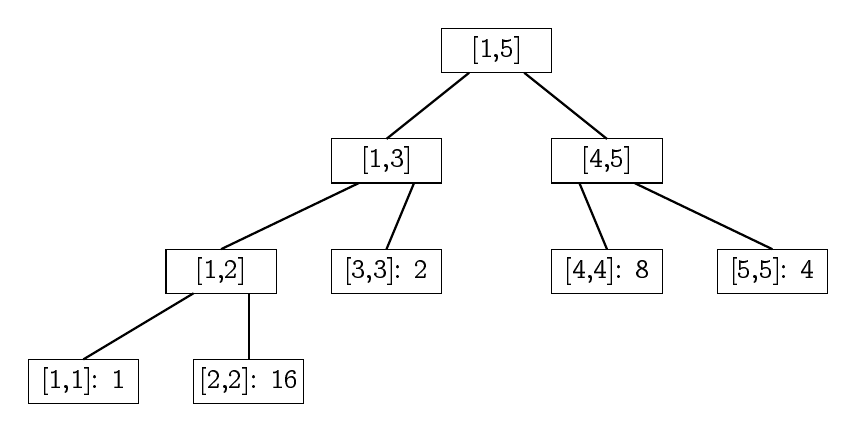
\begin{tikzpicture}[scale=0.7]
          \draw [black] (-1,7.9) rectangle (1,7.1) node [black, midway] {[1,5]}; % Draws a rectangle

          \draw [black] (-3,5.9) rectangle (-1,5.1) node [black,midway] {[1,3]}; % Draws a rectangle
          \draw [black] (1,5.9) rectangle (3,5.1) node [black,midway] {[4,5]}; % Draws a rectangle

          \draw [black] (-6,3.9) rectangle (-4,3.1) node [black,midway] {[1,2]}; % Draws a rectangle
          \draw [black] (-3,3.9) rectangle (-1,3.1) node [black,midway] {[3,3]: 2}; % Draws a rectangle
          \draw [black] (1,3.9) rectangle (3,3.1) node [black,midway] {[4,4]: 8}; % Draws a rectangle
          \draw [black] (4,3.9) rectangle (6,3.1) node [black,midway] {[5,5]: 4}; % Draws a rectangle

          \draw [black] (-8.5,1.9) rectangle (-6.5,1.1) node [black,midway] {[1,1]: 1}; % Draws a rectangle
          \draw [black] (-5.5,1.9) rectangle (-3.5,1.1) node [black,midway] {[2,2]: 16}; % Draws a rectangle

          \draw [thick] (-0.5,7.1) to (-2,5.9);
          \draw [thick] (0.5,7.1) to (2,5.9);

          \draw [thick] (-2.5,5.1) to (-5,3.9);
          \draw [thick] (-1.5,5.1) to (-2,3.9);

          \draw [thick] (1.5,5.1) to (2,3.9);
          \draw [thick] (2.5,5.1) to (5,3.9);

          \draw [thick] (-5.5,3.1) to (-7.5,1.9);
          \draw [thick] (-4.5,3.1) to (-4.5,1.9);
          % \draw [thick] (-2,2) % Draws a line
          % to [out=10,in=190] (2,2)
          % to [out=10,in=90] (6,0) 
          % to [out=-90,in=30] (-2,-2);    
        \end{tikzpicture}
      \end{figure}
  \end{itemize}
\end{frame}

\begin{frame}{基礎線段樹}
  \begin{itemize}
    \item 把這個結構存成樹,並假設每個節點都存該區間的最大值。以下假設 $a = [1, 16, 2, 8, 4]$
      \begin{figure}
        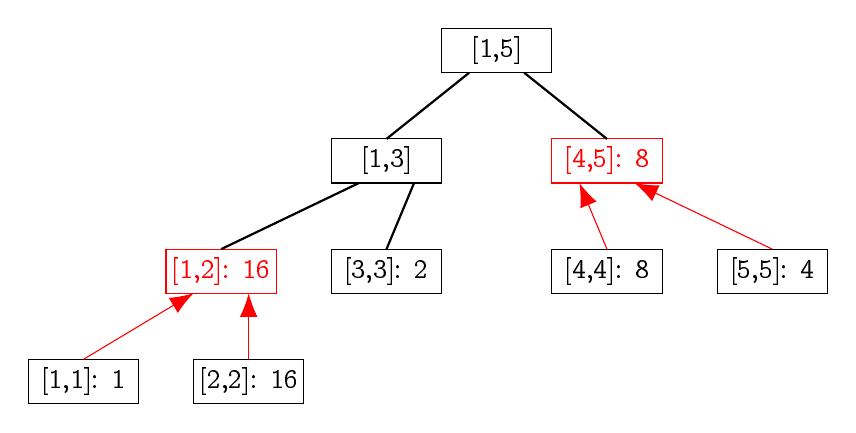
\begin{tikzpicture}[scale=0.7]
          \draw [black] (-1,7.9) rectangle (1,7.1) node [black, midway] {[1,5]}; % Draws a rectangle

          \draw [black] (-3,5.9) rectangle (-1,5.1) node [black,midway] {[1,3]}; % Draws a rectangle
          \draw [red] (1,5.9) rectangle (3,5.1) node [red,midway] {[4,5]: 8}; % Draws a rectangle

          \draw [red] (-6,3.9) rectangle (-4,3.1) node [red,midway] {[1,2]: 16}; % Draws a rectangle
          \draw [black] (-3,3.9) rectangle (-1,3.1) node [black,midway] {[3,3]: 2}; % Draws a rectangle
          \draw [black] (1,3.9) rectangle (3,3.1) node [black,midway] {[4,4]: 8}; % Draws a rectangle
          \draw [black] (4,3.9) rectangle (6,3.1) node [black,midway] {[5,5]: 4}; % Draws a rectangle

          \draw [black] (-8.5,1.9) rectangle (-6.5,1.1) node [black,midway] {[1,1]: 1}; % Draws a rectangle
          \draw [black] (-5.5,1.9) rectangle (-3.5,1.1) node [black,midway] {[2,2]: 16}; % Draws a rectangle

          \draw [thick] (-0.5,7.1) to (-2,5.9);
          \draw [thick] (0.5,7.1) to (2,5.9);

          \draw [thick] (-2.5,5.1) to (-5,3.9);
          \draw [thick] (-1.5,5.1) to (-2,3.9);

          \draw [red, arrows={Latex[length=3mm]}-] (1.5,5.1) -- (2,3.9);
          \draw [red, arrows={Latex[length=3mm]}-] (2.5,5.1) -- (5,3.9);

          \draw [red, arrows={Latex[length=3mm]}-] (-5.5,3.1) -- (-7.5,1.9);
          \draw [red, arrows={Latex[length=3mm]}-] (-4.5,3.1) -- (-4.5,1.9);
          % \draw [thick] (-2,2) % Draws a line
          % to [out=10,in=190] (2,2)
          % to [out=10,in=90] (6,0) 
          % to [out=-90,in=30] (-2,-2);    
        \end{tikzpicture}
      \end{figure}
  \end{itemize}
\end{frame}

\begin{frame}{基礎線段樹}
  \begin{itemize}
    \item 把這個結構存成樹,並假設每個節點都存該區間的最大值。以下假設 $a = [1, 16, 2, 8, 4]$
      \begin{figure}
        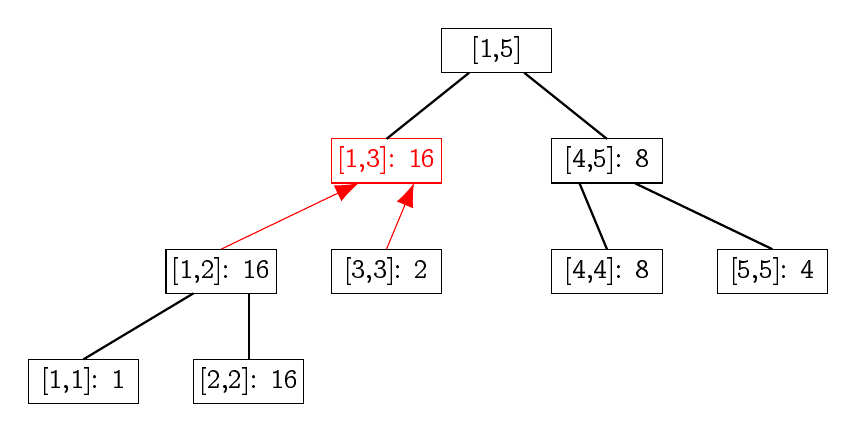
\begin{tikzpicture}[scale=0.7]
          \draw [black] (-1,7.9) rectangle (1,7.1) node [black, midway] {[1,5]}; % Draws a rectangle

          \draw [red] (-3,5.9) rectangle (-1,5.1) node [red,midway] {[1,3]: 16}; % Draws a rectangle
          \draw [black] (1,5.9) rectangle (3,5.1) node [black,midway] {[4,5]: 8}; % Draws a rectangle

          \draw [black] (-6,3.9) rectangle (-4,3.1) node [black,midway] {[1,2]: 16}; % Draws a rectangle
          \draw [black] (-3,3.9) rectangle (-1,3.1) node [black,midway] {[3,3]: 2}; % Draws a rectangle
          \draw [black] (1,3.9) rectangle (3,3.1) node [black,midway] {[4,4]: 8}; % Draws a rectangle
          \draw [black] (4,3.9) rectangle (6,3.1) node [black,midway] {[5,5]: 4}; % Draws a rectangle

          \draw [black] (-8.5,1.9) rectangle (-6.5,1.1) node [black,midway] {[1,1]: 1}; % Draws a rectangle
          \draw [black] (-5.5,1.9) rectangle (-3.5,1.1) node [black,midway] {[2,2]: 16}; % Draws a rectangle

          \draw [thick] (-0.5,7.1) to (-2,5.9);
          \draw [thick] (0.5,7.1) to (2,5.9);

          \draw [red, arrows={Latex[length=3mm]}-] (-2.5,5.1) -- (-5,3.9);
          \draw [red, arrows={Latex[length=3mm]}-] (-1.5,5.1) -- (-2,3.9);

          \draw [thick] (1.5,5.1) to (2,3.9);
          \draw [thick] (2.5,5.1) to (5,3.9);

          \draw [thick] (-5.5,3.1) to (-7.5,1.9);
          \draw [thick] (-4.5,3.1) to (-4.5,1.9);
          % \draw [thick] (-2,2) % Draws a line
          % to [out=10,in=190] (2,2)
          % to [out=10,in=90] (6,0) 
          % to [out=-90,in=30] (-2,-2);    
        \end{tikzpicture}
      \end{figure}
  \end{itemize}
\end{frame}

\begin{frame}{基礎線段樹}
  \begin{itemize}
    \item 把這個結構存成樹,並假設每個節點都存該區間的最大值。以下假設 $a = [1, 16, 2, 8, 4]$
      \begin{figure}
        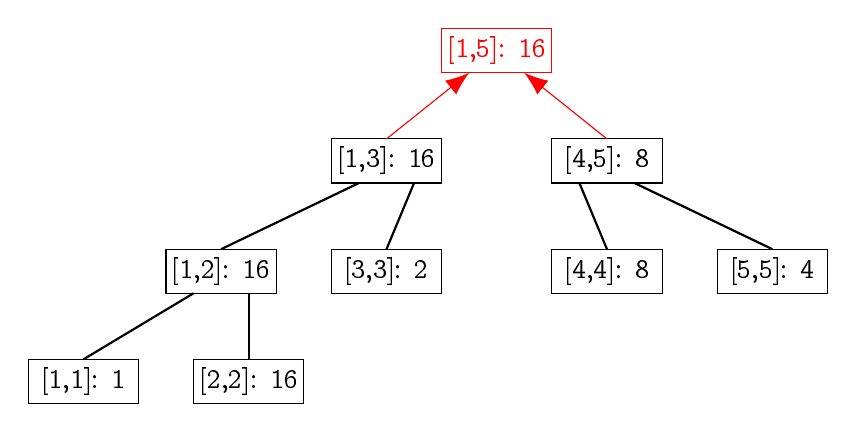
\begin{tikzpicture}[scale=0.7]
          \draw [red] (-1,7.9) rectangle (1,7.1) node [red, midway] {[1,5]: 16}; % Draws a rectangle

          \draw [black] (-3,5.9) rectangle (-1,5.1) node [black,midway] {[1,3]: 16}; % Draws a rectangle
          \draw [black] (1,5.9) rectangle (3,5.1) node [black,midway] {[4,5]: 8}; % Draws a rectangle

          \draw [black] (-6,3.9) rectangle (-4,3.1) node [black,midway] {[1,2]: 16}; % Draws a rectangle
          \draw [black] (-3,3.9) rectangle (-1,3.1) node [black,midway] {[3,3]: 2}; % Draws a rectangle
          \draw [black] (1,3.9) rectangle (3,3.1) node [black,midway] {[4,4]: 8}; % Draws a rectangle
          \draw [black] (4,3.9) rectangle (6,3.1) node [black,midway] {[5,5]: 4}; % Draws a rectangle

          \draw [black] (-8.5,1.9) rectangle (-6.5,1.1) node [black,midway] {[1,1]: 1}; % Draws a rectangle
          \draw [black] (-5.5,1.9) rectangle (-3.5,1.1) node [black,midway] {[2,2]: 16}; % Draws a rectangle

          \draw [red, arrows={Latex[length=3mm]}-] (-0.5,7.1) -- (-2,5.9);
          \draw [red, arrows={Latex[length=3mm]}-] (0.5,7.1) -- (2,5.9);

          \draw [thick] (-2.5,5.1) to (-5,3.9);
          \draw [thick] (-1.5,5.1) to (-2,3.9);

          \draw [thick] (1.5,5.1) to (2,3.9);
          \draw [thick] (2.5,5.1) to (5,3.9);

          \draw [thick] (-5.5,3.1) to (-7.5,1.9);
          \draw [thick] (-4.5,3.1) to (-4.5,1.9);
          % \draw [thick] (-2,2) % Draws a line
          % to [out=10,in=190] (2,2)
          % to [out=10,in=90] (6,0) 
          % to [out=-90,in=30] (-2,-2);    
        \end{tikzpicture}
      \end{figure}
  \end{itemize}
\end{frame}

\begin{frame}{基礎線段樹}
  \begin{itemize}
    \item $a = [1, 16, 2, 8, 4]$
      \begin{figure}
        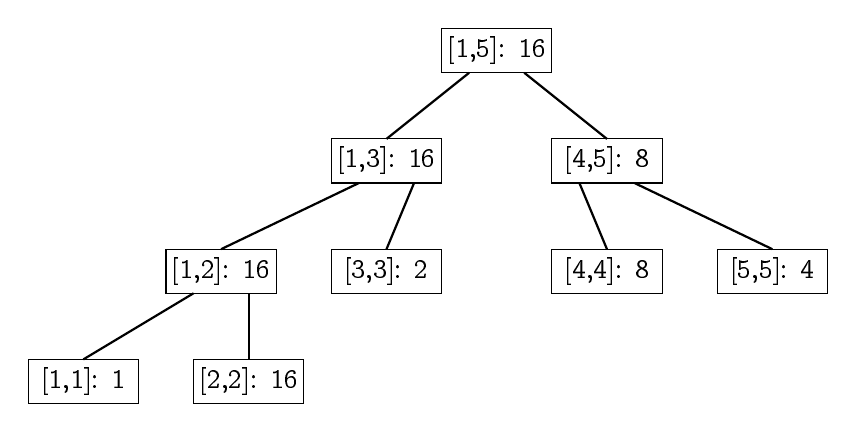
\begin{tikzpicture}[scale=0.7]
          \draw [black] (-1,7.9) rectangle (1,7.1) node [black, midway] {[1,5]: 16}; % Draws a rectangle

          \draw [black] (-3,5.9) rectangle (-1,5.1) node [black,midway] {[1,3]: 16}; % Draws a rectangle
          \draw [black] (1,5.9) rectangle (3,5.1) node [black,midway] {[4,5]: 8}; % Draws a rectangle

          \draw [black] (-6,3.9) rectangle (-4,3.1) node [black,midway] {[1,2]: 16}; % Draws a rectangle
          \draw [black] (-3,3.9) rectangle (-1,3.1) node [black,midway] {[3,3]: 2}; % Draws a rectangle
          \draw [black] (1,3.9) rectangle (3,3.1) node [black,midway] {[4,4]: 8}; % Draws a rectangle
          \draw [black] (4,3.9) rectangle (6,3.1) node [black,midway] {[5,5]: 4}; % Draws a rectangle

          \draw [black] (-8.5,1.9) rectangle (-6.5,1.1) node [black,midway] {[1,1]: 1}; % Draws a rectangle
          \draw [black] (-5.5,1.9) rectangle (-3.5,1.1) node [black,midway] {[2,2]: 16}; % Draws a rectangle

          \draw [thick] (-0.5,7.1) to (-2,5.9);
          \draw [thick] (0.5,7.1) to (2,5.9);

          \draw [thick] (-2.5,5.1) to (-5,3.9);
          \draw [thick] (-1.5,5.1) to (-2,3.9);

          \draw [thick] (1.5,5.1) to (2,3.9);
          \draw [thick] (2.5,5.1) to (5,3.9);

          \draw [thick] (-5.5,3.1) to (-7.5,1.9);
          \draw [thick] (-4.5,3.1) to (-4.5,1.9);
          % \draw [thick] (-2,2) % Draws a line
          % to [out=10,in=190] (2,2)
          % to [out=10,in=90] (6,0) 
          % to [out=-90,in=30] (-2,-2);    
        \end{tikzpicture}
      \end{figure}
    \item 答案是從某些預處理資料組合出來的:不知道可不可行
    \item 大資料都可以由小資料構成、小資料大小大概是大資料兩倍:可以
  \end{itemize}
\end{frame}

\begin{frame}{基礎線段樹}
  \begin{itemize}
    \item $a = [1, 16, 2, 8, 4]$
      \begin{figure}
        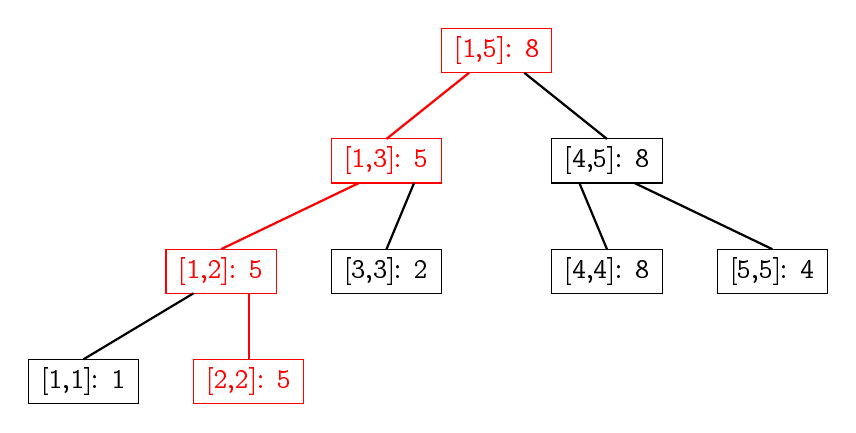
\begin{tikzpicture}[scale=0.7]
          \draw [red] (-1,7.9) rectangle (1,7.1) node [red, midway] {[1,5]: 8}; % Draws a rectangle

          \draw [red] (-3,5.9) rectangle (-1,5.1) node [red,midway] {[1,3]: 5}; % Draws a rectangle
          \draw [black] (1,5.9) rectangle (3,5.1) node [black,midway] {[4,5]: 8}; % Draws a rectangle

          \draw [red] (-6,3.9) rectangle (-4,3.1) node [red,midway] {[1,2]: 5}; % Draws a rectangle
          \draw [black] (-3,3.9) rectangle (-1,3.1) node [black,midway] {[3,3]: 2}; % Draws a rectangle
          \draw [black] (1,3.9) rectangle (3,3.1) node [black,midway] {[4,4]: 8}; % Draws a rectangle
          \draw [black] (4,3.9) rectangle (6,3.1) node [black,midway] {[5,5]: 4}; % Draws a rectangle

          \draw [black] (-8.5,1.9) rectangle (-6.5,1.1) node [black,midway] {[1,1]: 1}; % Draws a rectangle
          \draw [red] (-5.5,1.9) rectangle (-3.5,1.1) node [red,midway] {[2,2]: 5}; % Draws a rectangle

          \draw [thick, red] (-0.5,7.1) to (-2,5.9);
          \draw [thick] (0.5,7.1) to (2,5.9);

          \draw [thick, red] (-2.5,5.1) to (-5,3.9);
          \draw [thick] (-1.5,5.1) to (-2,3.9);

          \draw [thick] (1.5,5.1) to (2,3.9);
          \draw [thick] (2.5,5.1) to (5,3.9);

          \draw [thick] (-5.5,3.1) to (-7.5,1.9);
          \draw [thick, red] (-4.5,3.1) to (-4.5,1.9);
          % \draw [thick] (-2,2) % Draws a line
          % to [out=10,in=190] (2,2)
          % to [out=10,in=90] (6,0) 
          % to [out=-90,in=30] (-2,-2);    
        \end{tikzpicture}
      \end{figure}
    \item 修改一個元素的時候,讓包含這個元素的資料盡量少:好像可以(上圖是修改 $a_2$ 改成 $5$ 的狀況)
  \end{itemize}
\end{frame}

\begin{frame}{基礎線段樹}
  \begin{itemize}
    \item 在繼續下去之前,我們先來看看這棵樹的性質:
      \begin{itemize}
        \item 樹的節點總共有 $2N - 1$ 個
        \item 樹的高度為 $O(\log N)$
        \item 他是二元樹
      \end{itemize}
    \item 把樹上的數值填好只需要花 $O(N)$ 的時間(從葉子一路往上填,父節點的答案從左右子樹更新)
    \item 這種樹我們稱為「線段樹」
    \item 來看看怎麼把樹建出來吧!
  \end{itemize}
\end{frame}

\begin{frame}[fragile]{\btitle{範例實作}}
  \begin{minted}[breaklines]{cpp}
    const int inf = numeric_limits<int>::max();
    struct Node {
      Node *lc, *rc;
      int mx;
      void pull() { mx = max(lc->mx, rc->mx); }
    } *root = nullptr;
  \end{minted}

  \texttt{pull()} 這個函數用途是父節點利用左右子樹的答案更新自己的答案,\textbf{每當任何子樹的值有更動時,都需要重新呼叫這個 function 更新父節點的答案}
\end{frame}

\begin{frame}[fragile]{\btitle{範例實作}}
  \begin{minted}[breaklines]{cpp}
    Node *build(int arr[], int l, int r) { // 回傳區間 [l, r] 這段區間構成的線段樹的根節點
      Node *res = new Node();
      if (l == r) { // 葉節點
        res->lc = res->rc = nullptr;
        res->mx = arr[l];
      } else {
        int m = (l + r) / 2;
        res->lc = build(arr, l, m); // 把左半區間建好的樹接在自己的左子樹上
        res->rc = build(arr, m + 1, r); // 把右半區間建好的樹接在自己的左子樹上
        res->pull(); // 更新父節點資訊
      }
      return res;
    }
  \end{minted}
\end{frame}

\begin{frame}[fragile]{\btitle{範例實作}}
  \begin{itemize}
    \item 線段樹的實作會使用到大量的遞迴!
    \item 在遞迴線段樹節點的時候,通常會把該節點代表的區間(上述 code 的 $l, r$)一起遞迴下去
    \item 線段樹的實作有很多種版本,這裡提供的是指標版
  \end{itemize}
\end{frame}

\begin{frame}{基礎線段樹}
  \begin{itemize}
    \item $a = [1, 16, 2, 8, 4]$
      \begin{figure}
        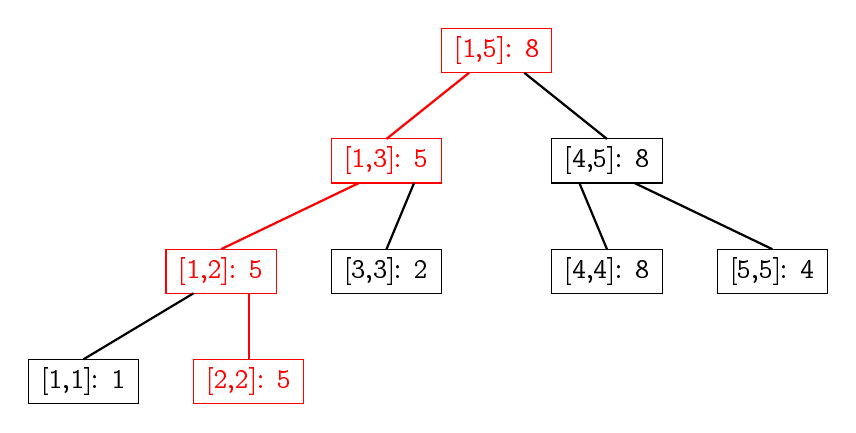
\begin{tikzpicture}[scale=0.7]
          \draw [red] (-1,7.9) rectangle (1,7.1) node [red, midway] {[1,5]: 8}; % Draws a rectangle

          \draw [red] (-3,5.9) rectangle (-1,5.1) node [red,midway] {[1,3]: 5}; % Draws a rectangle
          \draw [black] (1,5.9) rectangle (3,5.1) node [black,midway] {[4,5]: 8}; % Draws a rectangle

          \draw [red] (-6,3.9) rectangle (-4,3.1) node [red,midway] {[1,2]: 5}; % Draws a rectangle
          \draw [black] (-3,3.9) rectangle (-1,3.1) node [black,midway] {[3,3]: 2}; % Draws a rectangle
          \draw [black] (1,3.9) rectangle (3,3.1) node [black,midway] {[4,4]: 8}; % Draws a rectangle
          \draw [black] (4,3.9) rectangle (6,3.1) node [black,midway] {[5,5]: 4}; % Draws a rectangle

          \draw [black] (-8.5,1.9) rectangle (-6.5,1.1) node [black,midway] {[1,1]: 1}; % Draws a rectangle
          \draw [red] (-5.5,1.9) rectangle (-3.5,1.1) node [red,midway] {[2,2]: 5}; % Draws a rectangle

          \draw [thick, red] (-0.5,7.1) to (-2,5.9);
          \draw [thick] (0.5,7.1) to (2,5.9);

          \draw [thick, red] (-2.5,5.1) to (-5,3.9);
          \draw [thick] (-1.5,5.1) to (-2,3.9);

          \draw [thick] (1.5,5.1) to (2,3.9);
          \draw [thick] (2.5,5.1) to (5,3.9);

          \draw [thick] (-5.5,3.1) to (-7.5,1.9);
          \draw [thick, red] (-4.5,3.1) to (-4.5,1.9);
          % \draw [thick] (-2,2) % Draws a line
          % to [out=10,in=190] (2,2)
          % to [out=10,in=90] (6,0) 
          % to [out=-90,in=30] (-2,-2);    
        \end{tikzpicture}
      \end{figure}
    \item 單點修改其實只會從\textbf{葉節點一路修改到根}
    \item 樹高是 $O(\log N)$,所以複雜度為 $O(\log N)$
  \end{itemize}
\end{frame}

\begin{frame}{\btitle{修改二步驟}}
  \begin{itemize}
    \item 修改的位置是 \(p\)
    \item 假設目前的節點儲存的資訊是 \([L, R]\)
    \item 修改二步驟:
    \begin{enumerate}
      \item
        如果 \([L, R]\) 區間長度為 1,可以知道這就是是一個葉節點。
      \item
          否則設 \(M = \lfloor \frac{L+R}{2} \rfloor\),\(p\) 一定在 \([L, M]\) 或是 \([M+1, R]\) 其中之一,依照 \(p\) 與 \(M\) 的關係決定往哪個子樹遞迴。
          在子樹更新完之後,\textbf{更新這個節點的最大值}成為兩個子節點當中較大的。
    \end{enumerate}
  \end{itemize}
\end{frame}

\begin{frame}[fragile]{\btitle{範例實作}}
  \begin{minted}[breaklines]{cpp}
    void modify(Node *nd, int val, int p, int l, int r) {
      if (l == r) { // 葉節點
        nd->mx = val;
        return;
      }
      int m = (l + r) / 2;
      if (p <= m) // 看修改的點是在左邊還是右邊
        modify(nd->lc, val, p, l, m);
      else
        modify(nd->rc, val, p, m + 1, r);
      nd->pull(); // IMPORTANT!!
    }
  \end{minted}
\end{frame}

\begin{frame}[fragile]{\btitle{查詢}}
  \begin{itemize}
    \item 查詢 $[3, 5]$
      \begin{figure}
        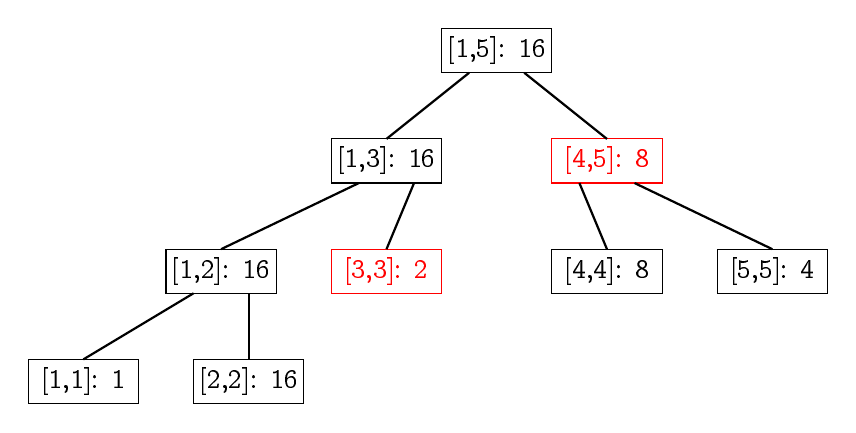
\begin{tikzpicture}[scale=0.7]
          \draw [black] (-1,7.9) rectangle (1,7.1) node [black, midway] {[1,5]: 16}; % Draws a rectangle

          \draw [black] (-3,5.9) rectangle (-1,5.1) node [black,midway] {[1,3]: 16}; % Draws a rectangle
          \draw [red] (1,5.9) rectangle (3,5.1) node [red,midway] {[4,5]: 8}; % Draws a rectangle

          \draw [black] (-6,3.9) rectangle (-4,3.1) node [black,midway] {[1,2]: 16}; % Draws a rectangle
          \draw [red] (-3,3.9) rectangle (-1,3.1) node [red,midway] {[3,3]: 2}; % Draws a rectangle
          \draw [black] (1,3.9) rectangle (3,3.1) node [black,midway] {[4,4]: 8}; % Draws a rectangle
          \draw [black] (4,3.9) rectangle (6,3.1) node [black,midway] {[5,5]: 4}; % Draws a rectangle

          \draw [black] (-8.5,1.9) rectangle (-6.5,1.1) node [black,midway] {[1,1]: 1}; % Draws a rectangle
          \draw [black] (-5.5,1.9) rectangle (-3.5,1.1) node [black,midway] {[2,2]: 16}; % Draws a rectangle

          \draw [thick] (-0.5,7.1) to (-2,5.9);
          \draw [thick] (0.5,7.1) to (2,5.9);

          \draw [thick] (-2.5,5.1) to (-5,3.9);
          \draw [thick] (-1.5,5.1) to (-2,3.9);

          \draw [thick] (1.5,5.1) to (2,3.9);
          \draw [thick] (2.5,5.1) to (5,3.9);

          \draw [thick] (-5.5,3.1) to (-7.5,1.9);
          \draw [thick] (-4.5,3.1) to (-4.5,1.9);
          % \draw [thick] (-2,2) % Draws a line
          % to [out=10,in=190] (2,2)
          % to [out=10,in=90] (6,0) 
          % to [out=-90,in=30] (-2,-2);    
        \end{tikzpicture}
      \end{figure}
  \end{itemize}
\end{frame}

\begin{frame}[fragile]{\btitle{查詢}}
  \begin{itemize}
    \item 查詢 $[1, 4]$
      \begin{figure}
        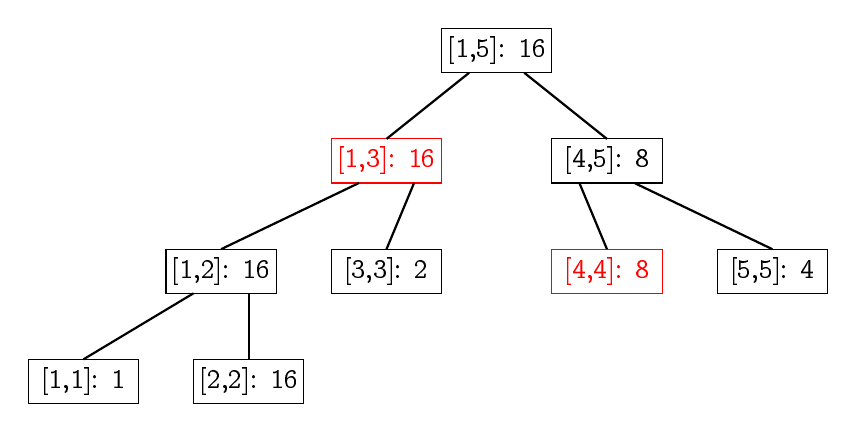
\begin{tikzpicture}[scale=0.7]
          \draw [black] (-1,7.9) rectangle (1,7.1) node [black, midway] {[1,5]: 16}; % Draws a rectangle

          \draw [red] (-3,5.9) rectangle (-1,5.1) node [red,midway] {[1,3]: 16}; % Draws a rectangle
          \draw [black] (1,5.9) rectangle (3,5.1) node [black,midway] {[4,5]: 8}; % Draws a rectangle

          \draw [black] (-6,3.9) rectangle (-4,3.1) node [black,midway] {[1,2]: 16}; % Draws a rectangle
          \draw [black] (-3,3.9) rectangle (-1,3.1) node [black,midway] {[3,3]: 2}; % Draws a rectangle
          \draw [red] (1,3.9) rectangle (3,3.1) node [red,midway] {[4,4]: 8}; % Draws a rectangle
          \draw [black] (4,3.9) rectangle (6,3.1) node [black,midway] {[5,5]: 4}; % Draws a rectangle

          \draw [black] (-8.5,1.9) rectangle (-6.5,1.1) node [black,midway] {[1,1]: 1}; % Draws a rectangle
          \draw [black] (-5.5,1.9) rectangle (-3.5,1.1) node [black,midway] {[2,2]: 16}; % Draws a rectangle

          \draw [thick] (-0.5,7.1) to (-2,5.9);
          \draw [thick] (0.5,7.1) to (2,5.9);

          \draw [thick] (-2.5,5.1) to (-5,3.9);
          \draw [thick] (-1.5,5.1) to (-2,3.9);

          \draw [thick] (1.5,5.1) to (2,3.9);
          \draw [thick] (2.5,5.1) to (5,3.9);

          \draw [thick] (-5.5,3.1) to (-7.5,1.9);
          \draw [thick] (-4.5,3.1) to (-4.5,1.9);
          % \draw [thick] (-2,2) % Draws a line
          % to [out=10,in=190] (2,2)
          % to [out=10,in=90] (6,0) 
          % to [out=-90,in=30] (-2,-2);    
        \end{tikzpicture}
      \end{figure}
    \item 好像可以由蠻少數量的區間得到答案ㄋㄟ,可是具體是多小呢?
  \end{itemize}
\end{frame}

\begin{frame}{\btitle{查詢}}
  \begin{itemize}
    \item 把選法說的具體一點:
      \begin{itemize}
        \item 從根往下看
        \item 每當看到一個被詢問區間完全包含的節點時,就直接使用該節點的答案
        \item 否則就嘗試左右遞迴取出比較好的區間
      \end{itemize}
  \end{itemize}
\end{frame}

\begin{frame}{\btitle{查詢三步驟}}
  \begin{itemize}
    \item 目標:區間詢問 \([ql,qr]\)(\(ql \leq qr\)) 的最大值
    \item 假設目前的節點儲存的資訊是 \([L, R]\)
    \item 查詢三步驟:
    \begin{enumerate}
      \item
        如果 \([L, R]\) 完整的被 \([ql, qr]\) 包含,即 \(ql \leq L \leq R \leq qr\),那麼我們可以直接取用這個節點的最大值。
      \item
        如果 \([L, R]\) 完全跟 \([ql, qr]\) 沒有交集,那麼可以退出遞迴了。
      \item
        否則,遞迴往兩個子樹求解。
    \end{enumerate}
  \end{itemize}
\end{frame}

\begin{frame}{\btitle{查詢三步驟}}
  \begin{itemize}
    \item 複雜度是多少呢?
    \item 很神奇的是,答案可以由 $O(\log N)$ 個預處理資料得到,並且從根走到 + 走完這 $O(\log N)$ 個資料還是 $O(\log N)$
    \item 很神奇的結論!證明記不起來沒關係
    \item \textbf{這就是線段樹的精隨:他可以把一個大區間拆成 $O(\log N)$ 個小區間!}
  \end{itemize}
\end{frame}

\begin{frame}{\btitle{查詢時間複雜度證明}}
  \begin{itemize}
    \item 先找到一個節點 $M$,詢問區間的所有值都在以這個節點為根的子樹裡面,而且這個點要盡量的深(白話文:盡量剛剛好包住詢問區間)
    \begin{itemize}
      \item 從根走到 $M$ 路上只會一直 3.
      \item 用 3. 之後的左右子樹,一個會進到 3.,另外一個進到 2.
      \item 樹深最多 $O(\log N)$,因此最多只會碰到 $O(\log N)$ 個節點
    \end{itemize}
    \item 從 $M$ 開始後,查詢區間其實就被切成左半邊跟右半邊。
    \item 左半邊其實是從 $M$ 的 $mid$ 往左的某段後綴
    \item 右半邊其實是從 $M$ 的 $mid + 1$ 往右的某段前綴
    \item 而後綴 / 前綴的好處是,每當 3. 發生時,左右子樹一定至少有一個是 1. 或 2.
    \item 而 3. 在每個深度最多只會發生一次,所以整題複雜度還是 $O(\log N)$
    \item 整體而言,詢問區間只需要由 $O(\log N)$ 個小區間構成,而造訪這些小區間的複雜度也是 $O(\log N)$!
  \end{itemize}
\end{frame}

\begin{frame}[fragile]{\btitle{範例實作}}
  \begin{minted}[breaklines]{cpp}
    int query(Node *nd, int ql, int qr, int l, int r) {
      if (r < ql || l > qr)   // 完全不包含
        return -inf;
      if (ql <= l && r <= qr) // 完全包含
        return nd->mx;
      int m = (l + r) / 2;
      return max(query(nd->lc, ql, qr, l, m), query(nd->rc, ql, qr, m + 1, r)); // 左右遞迴
    }
  \end{minted}
\end{frame}

\end{document}


\documentclass[standalone]{beamer}

\begin{document}
\section{BIT}

\begin{frame}{BIT}
  \begin{itemize}
    \item Binary Indexed Tree
    \item Fenwick Tree
    \item 樹狀數組
    \item 支援操作:單點加值、前綴求和
  \end{itemize}
\end{frame}

\begin{frame}{BIT}
  \begin{itemize}
    \item 我們有一個陣列 $a[1\ldots n]$,以及另一個陣列 $s[1\ldots n]$
    \item $s[i]$ 紀錄的是 $\sum_{j=i-lowbit(i)+1}^{i}{a[j]}$
    \item $lowbit(x)$ 的值是 $x$ 寫成二進位時最小的一個 1-bit 的值
    \item 比如說,$44 = 101100_2, lowbit(44) = 2^2 = 4$
    \item $lowbit(x) = x \& (-x)$
    \item 好抽象,來看圖吧!
  \end{itemize}
\end{frame}

\begin{frame}{BIT}
  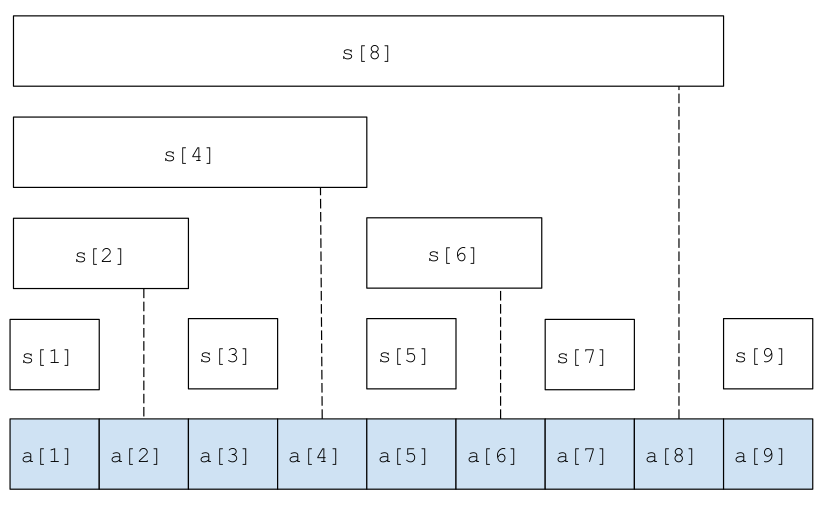
\includegraphics[width=10cm]{figures/bit.png}

  有沒有很像沒有右邊子樹的線段樹!
\end{frame}

\begin{frame}{\btitle{前綴求和}}
  \begin{itemize}
    \item 假設要求 $a[1...46]$
    \item $= s[46] + a[1...44]$
    \item $= s[46] + s[44] + a[1...40]$
    \item 有發現什麼嗎?
    \item 令 $sum(x)=a[1]+a[2]+\cdots+a[x-1]+a[x]$
    \item 前面好像就只是 $sum(x) = s[x] + sum(x - lowbit(x))$
    \item 遞迴求 $sum(x)$!
  \end{itemize}
\end{frame}

\begin{frame}[fragile]{\btitle{前綴求和}}
  \begin{minted}[breaklines]{cpp}
    int sum(int id) {
      int res = 0;
      for (int i = id; i > 0; i -= i & -i)
        res += s[i];
      return res;
    }
  \end{minted}
\end{frame}

\begin{frame}{\btitle{單點加值}}
  \begin{itemize}
    \item 假設要把 $a[46]$ 加上 $x$,把有蓋到 $46$ 的值加上去就好了
    \item 首先觀察發現有蓋到 46 的節點編號一定不小於 46 ,畢竟節點 $i$ 蓋到的區間是 $(i-lowbit(i),i]$
    \item 其實古人的智慧告訴我們,會蓋到 $i$ 的區間編號其實就是以下的序列:
    \item $\{s_0 = i, s_{k+1} = s_k + lowbit(s_k)\}$ ,一直到 $s_k > N$ 為止
      \begin{itemize}
        \item 簡單小證明:
        \item $lowbit(s_{k + 1}) > lowbit(s_k)$,所以 $s_{k + 1}$ 會覆蓋到 $s_k$ 覆蓋的範圍
        \item 而 $s_{k + 1}$ 恰好是所有覆蓋 $s_k$ 範圍中最小的那一個
      \end{itemize}
  \end{itemize}
\end{frame}

\begin{frame}[fragile]{\btitle{前綴求和}}
  \begin{minted}[breaklines]{cpp}
    void upd(int id, int x) {
      for (int i = id; i <= n; i += i & -i)
        s[i] += x;
    }
  \end{minted}
\end{frame}

\begin{frame}{\btitle{單點加值、區間求和}}
  \begin{itemize}
    \item 有了這些,就可以解決一個很常見的問題了:單點加值、區間求和
    \item 單點加值 $a_i += x$ 直接 \texttt{upd(i, x);} 就好
    \item 區間求和 $[l, r]$ 其實可以用前綴和的方式得到:\texttt{sum(r) - sum(l - 1);}
  \end{itemize}
\end{frame}

\begin{frame}{\btitle{第 K 小}}
  \begin{itemize}
    \item 假設 $a[x]$ 是存 $x$ 這個數字出現過幾次
    \item 那 $sum(i)$ 就是 $\le i$ 的元素有幾個
    \item $i$ 是集合裡第 $k$ 小的元素若且唯若 $sum(i - 1) < k$ 且 $sum(i) \ge k$
    \item 二分搜!
    \item 直接呼叫 query 二分搜是 $O(\log^2 N)$,複雜度似乎不太好
    \item 用 BIT 的結構在上面二分搜!
  \end{itemize}
\end{frame}

\begin{frame}{\btitle{第 K 小}}
  來看圖!

  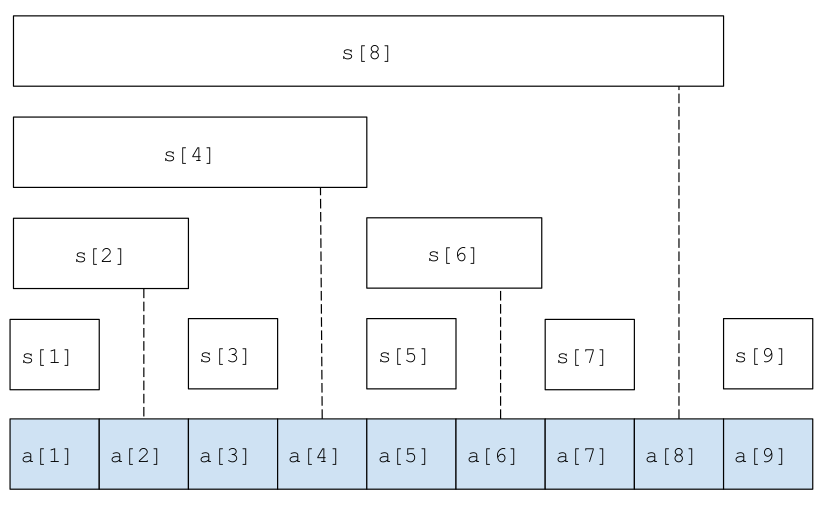
\includegraphics[width=10cm]{figures/bit.png}
\end{frame}


\begin{frame}[fragile]{\btitle{第 K 小}}
  \begin{minted}[breaklines]{cpp}
    int kth(int k) {
      int res = 0;
      for (int i = 1 << __lg(n); i > 0; i >>= 1)
        // 決定 res 應該在 [res, res + i - 1] 還是 [res + i, res + 2i - 1]
        if (res + i <= n && dat[res + i] < k) // 左邊的個數不夠,往右邊走
          k -= dat[res += i];
        // 否則就代表左邊其實是夠的,就往左邊走
      return res + 1;
    }
  \end{minted}
\end{frame}

\begin{frame}{\btitle{BIT 與差分}}
  \begin{itemize}
    \item 差分序列:$d_i = a_i - a_{i - 1}$
    \item 如果 BIT 維護差分序列的話,就可以變成支援區間加值、單點求值的資料結構
    \item $a_i = d_1 + d_2 + \ldots + d_i$
    \item 把 $a_l, \ldots, a_r$ 全部加上 $x$,相對應在差分數列上的變化其實只是 $d_l$ 加上 $x$,$d_{r+1}$ 扣掉 $x$
  \end{itemize}
\end{frame}

\begin{frame}{\btitle{總結}}
  \begin{itemize}
    \item 支援單點修改、前綴求和、查詢第 k 小的資料結構
    \item 常數很小、寫起來比線段樹簡單許多
    \item 實用!
  \end{itemize}
\end{frame}

\end{document}


\documentclass[standalone]{beamer}

\begin{document}
\section{進階線段樹}

\begin{frame}[fragile]{進階線段樹}
  \begin{itemize}
    \item 來看看強大的線段樹可以做些什麼吧~
    \item 這裡講的技巧只是線段樹強大應用中的冰山一角,有興趣的讀者可以閱讀進階資料結構講義,或者是自行上網搜尋更加進階的應用喔!
  \end{itemize}
\end{frame}

\begin{frame}[fragile]{\btitle{精妙狀態合併}}
  \begin{itemize}
    \item 線段樹不僅可以維護簡單的最大最小值或總和,只要能夠快速從左右子區間的資訊得知合併後的區間的所有資訊的問題,就可以用線段樹解決
    \item 來看例題!
    \begin{problem}[區間最大連續和]
      給定長度為 \(N\) 的序列 \(a_1, a_2, \dots, a_N\),接著有 \(Q\) 個形如 \(\texttt{l r}\) 的詢問,請你回答 \(a_l, a_{l+1}, \dots, a_r\) 這個序列的最大連續和。

      \begin{itemize}
          \item
              \(N, Q \leq 5 \times 10^5\)
      \end{itemize}
    \end{problem}
  \end{itemize}
\end{frame}

\begin{frame}[fragile]{\btitle{精妙狀態合併}}
  \begin{itemize}
    \item 想想看怎麼用分治法求出最大連續和!
    \item 在線段樹每個節點上,我們可以維護以下資訊:
      \begin{itemize}
          \item 以區間最左端為左界的最大連續和,即最大總和的前綴。
          \item 以區間最右端為右界的最大連續和,即最大總和的後綴。
          \item 整個區間的最大連續和。
          \item 整個區間的總和。
      \end{itemize}
    \item 所有的區間可以分成三種:通過區間中點、完全落在左半區間、完全落在右半區間
    \item 中點的最大連續和一定是左半區間的最大後綴加上右半區間的最大前綴
  \end{itemize}
\end{frame}

\begin{frame}[fragile]{\btitle{精妙狀態合併}}
  \begin{minted}[breaklines]{cpp}
    struct Info {
      int64_t sum, lmx, rmx, mx;
    };
    Info combine(const Info &lhs, const Info &rhs) {
      Info res;
      res.sum = lhs.sum + rhs.sum;
      res.lmx = max(lhs.lmx, lhs.sum + rhs.lmx);
      res.rmx = max(lhs.rmx + rhs.sum, rhs.rmx);
      res.mx = max({lhs.mx, rhs.mx, lhs.rmx + rhs.lmx});
      return res;
    }
  \end{minted}
\end{frame}

\begin{frame}[fragile]{\btitle{懶人標記}}
  \begin{itemize}
    \item 直接來看例題!
    \begin{problem}[區間加值、區間最大值]
      給定一個長度為 \(N\) 的正整數序列 \(a_1, \dots, a_N\),接著有 \(Q\) 個詢問,每個詢問形如
      \begin{itemize}
          \item
              \(\texttt{1 l r}\),請輸出 \(a_l, a_{l+1}, \dots, a_r\) 當中最大的數字是多少。
          \item
              \(\texttt{2 l r d}\),讓 \(a_l, a_{l+1}, \dots, a_r\) 全部增加 \(d\)。
      \end{itemize}

      \begin{itemize}
          \item \(N, Q \leq 5 \times 10^5\)
          \item \(d > 0\)
      \end{itemize}
    \end{problem}
  \end{itemize}
\end{frame}

\begin{frame}[fragile]{\btitle{懶人標記}}
  \begin{itemize}
    \item 如果這題只是單純做 $r - l + 1$ 次單點修改的話,修改的複雜度會退化成 $O(N \log N)$
    \item 有沒有辦法把修改的區間拆成 $O(\log N)$ 個區間,並對每個區間做一些事情後,就達到修改的效果呢?
    \item 可以!
  \end{itemize}
\end{frame}

\begin{frame}[fragile]{\btitle{懶人標記}}
  \begin{itemize}
    \item 每個節點上面存一個「標記」,表示被\textbf{這個節點對應的區間涵蓋的所有元素都必須加上某個值}
    \item 在區間修改時,我們就在所有區間打上這樣的「標記」
    \item 在打標記的時候,同時修改該節點的資訊,並且一路 pull 回去!
  \end{itemize}
\end{frame}

\begin{frame}[fragile]{\btitle{懶人標記}}
  \begin{itemize}
    \item $a = [1, 16, 2, 8, 4]$,並把 $[1, 4]$ 加上 $3$
    \item 先把 tag 打上去!
      \begin{figure}
        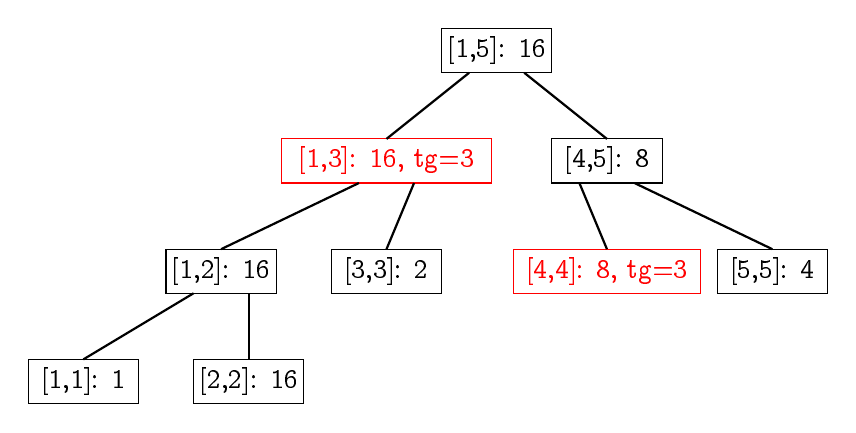
\begin{tikzpicture}[scale=0.7]
          \draw [black] (-1,7.9) rectangle (1,7.1) node [black, midway] {[1,5]: 16}; % Draws a rectangle

          \draw [red] (-3.9,5.9) rectangle (-0.1,5.1) node [red,midway] {[1,3]: 16, tg=3}; % Draws a rectangle
          \draw [black] (1,5.9) rectangle (3,5.1) node [black,midway] {[4,5]: 8}; % Draws a rectangle

          \draw [black] (-6,3.9) rectangle (-4,3.1) node [black,midway] {[1,2]: 16}; % Draws a rectangle
          \draw [black] (-3,3.9) rectangle (-1,3.1) node [black,midway] {[3,3]: 2}; % Draws a rectangle
          \draw [red] (0.3,3.9) rectangle (3.7,3.1) node [red,midway] {[4,4]: 8, tg=3}; % Draws a rectangle
          \draw [black] (4,3.9) rectangle (6,3.1) node [black,midway] {[5,5]: 4}; % Draws a rectangle

          \draw [black] (-8.5,1.9) rectangle (-6.5,1.1) node [black,midway] {[1,1]: 1}; % Draws a rectangle
          \draw [black] (-5.5,1.9) rectangle (-3.5,1.1) node [black,midway] {[2,2]: 16}; % Draws a rectangle

          \draw [thick] (-0.5,7.1) to (-2,5.9);
          \draw [thick] (0.5,7.1) to (2,5.9);

          \draw [thick] (-2.5,5.1) to (-5,3.9);
          \draw [thick] (-1.5,5.1) to (-2,3.9);

          \draw [thick] (1.5,5.1) to (2,3.9);
          \draw [thick] (2.5,5.1) to (5,3.9);

          \draw [thick] (-5.5,3.1) to (-7.5,1.9);
          \draw [thick] (-4.5,3.1) to (-4.5,1.9);
          % \draw [thick] (-2,2) % Draws a line
          % to [out=10,in=190] (2,2)
          % to [out=10,in=90] (6,0) 
          % to [out=-90,in=30] (-2,-2);    
        \end{tikzpicture}
      \end{figure}
  \end{itemize}
\end{frame}

\begin{frame}[fragile]{\btitle{懶人標記}}
  \begin{itemize}
    \item $a = [1, 16, 2, 8, 4]$,並把 $[1, 4]$ 加上 $3$
    \item 更新被打 tag 的區間的答案
      \begin{figure}
        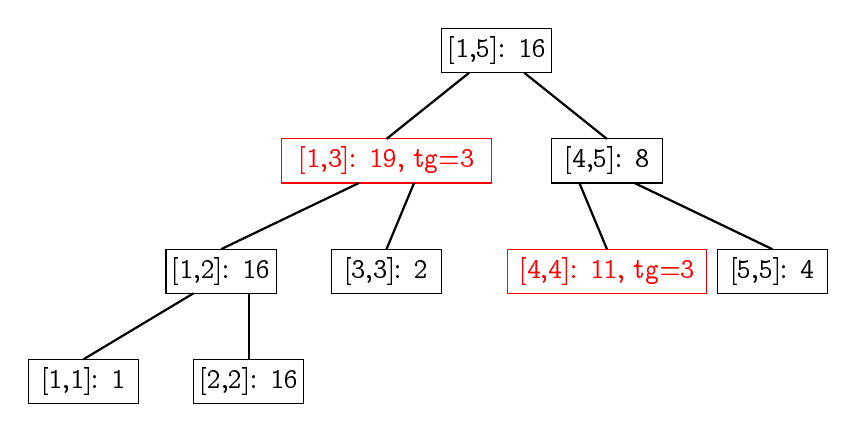
\begin{tikzpicture}[scale=0.7]
          \draw [black] (-1,7.9) rectangle (1,7.1) node [black, midway] {[1,5]: 16}; % Draws a rectangle

          \draw [red] (-3.9,5.9) rectangle (-0.1,5.1) node [red,midway] {[1,3]: 19, tg=3}; % Draws a rectangle
          \draw [black] (1,5.9) rectangle (3,5.1) node [black,midway] {[4,5]: 8}; % Draws a rectangle

          \draw [black] (-6,3.9) rectangle (-4,3.1) node [black,midway] {[1,2]: 16}; % Draws a rectangle
          \draw [black] (-3,3.9) rectangle (-1,3.1) node [black,midway] {[3,3]: 2}; % Draws a rectangle
          \draw [red] (0.2,3.9) rectangle (3.8,3.1) node [red,midway] {[4,4]: 11, tg=3}; % Draws a rectangle
          \draw [black] (4,3.9) rectangle (6,3.1) node [black,midway] {[5,5]: 4}; % Draws a rectangle

          \draw [black] (-8.5,1.9) rectangle (-6.5,1.1) node [black,midway] {[1,1]: 1}; % Draws a rectangle
          \draw [black] (-5.5,1.9) rectangle (-3.5,1.1) node [black,midway] {[2,2]: 16}; % Draws a rectangle

          \draw [thick] (-0.5,7.1) to (-2,5.9);
          \draw [thick] (0.5,7.1) to (2,5.9);

          \draw [thick] (-2.5,5.1) to (-5,3.9);
          \draw [thick] (-1.5,5.1) to (-2,3.9);

          \draw [thick] (1.5,5.1) to (2,3.9);
          \draw [thick] (2.5,5.1) to (5,3.9);

          \draw [thick] (-5.5,3.1) to (-7.5,1.9);
          \draw [thick] (-4.5,3.1) to (-4.5,1.9);
          % \draw [thick] (-2,2) % Draws a line
          % to [out=10,in=190] (2,2)
          % to [out=10,in=90] (6,0) 
          % to [out=-90,in=30] (-2,-2);    
        \end{tikzpicture}
      \end{figure}
  \end{itemize}
\end{frame}

\begin{frame}[fragile]{\btitle{懶人標記}}
  \begin{itemize}
    \item $a = [1, 16, 2, 8, 4]$,並把 $[1, 4]$ 加上 $3$
    \item pull 回 root!
      \begin{figure}
        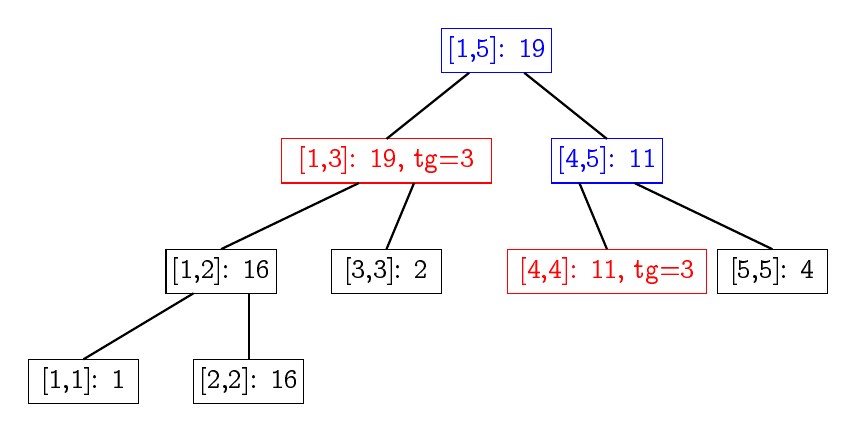
\begin{tikzpicture}[scale=0.7]
          \draw [blue] (-1,7.9) rectangle (1,7.1) node [blue, midway] {[1,5]: 19}; % Draws a rectangle

          \draw [red] (-3.9,5.9) rectangle (-0.1,5.1) node [red,midway] {[1,3]: 19, tg=3}; % Draws a rectangle
          \draw [blue] (1,5.9) rectangle (3,5.1) node [blue,midway] {[4,5]: 11}; % Draws a rectangle

          \draw [black] (-6,3.9) rectangle (-4,3.1) node [black,midway] {[1,2]: 16}; % Draws a rectangle
          \draw [black] (-3,3.9) rectangle (-1,3.1) node [black,midway] {[3,3]: 2}; % Draws a rectangle
          \draw [red] (0.2,3.9) rectangle (3.8,3.1) node [red,midway] {[4,4]: 11, tg=3}; % Draws a rectangle
          \draw [black] (4,3.9) rectangle (6,3.1) node [black,midway] {[5,5]: 4}; % Draws a rectangle

          \draw [black] (-8.5,1.9) rectangle (-6.5,1.1) node [black,midway] {[1,1]: 1}; % Draws a rectangle
          \draw [black] (-5.5,1.9) rectangle (-3.5,1.1) node [black,midway] {[2,2]: 16}; % Draws a rectangle

          \draw [thick] (-0.5,7.1) to (-2,5.9);
          \draw [thick] (0.5,7.1) to (2,5.9);

          \draw [thick] (-2.5,5.1) to (-5,3.9);
          \draw [thick] (-1.5,5.1) to (-2,3.9);

          \draw [thick] (1.5,5.1) to (2,3.9);
          \draw [thick] (2.5,5.1) to (5,3.9);

          \draw [thick] (-5.5,3.1) to (-7.5,1.9);
          \draw [thick] (-4.5,3.1) to (-4.5,1.9);
          % \draw [thick] (-2,2) % Draws a line
          % to [out=10,in=190] (2,2)
          % to [out=10,in=90] (6,0) 
          % to [out=-90,in=30] (-2,-2);    
        \end{tikzpicture}
      \end{figure}
  \end{itemize}
\end{frame}

\begin{frame}[fragile]{\btitle{懶人標記}}
  \begin{itemize}
    \item 一些發現:
      \begin{itemize}
        \item 有打 tag 的節點的父親們的答案都是正確的
        \item tag 底下的節點還沒有被更新到,但如果沒碰到他們的話,他們其實也不用被更新(?)
        \item 有 tag 要更新答案很簡單
      \end{itemize}
    \item 標記的關鍵:\textbf{需要的時候再去更新,沒需要就不要管他}
    \item 如果有兩個標記撞在一起,把他加起來就好了(標記很好合併)!
    \item 那,什麼時候是\textbf{需要的時候}?
  \end{itemize}
\end{frame}

\begin{frame}[fragile]{\btitle{懶人標記}}
  \begin{itemize}
    \item 那,什麼時候是\textbf{需要的時候}?
    \item 注意到標記的特性:這個節點對應的區間涵蓋的所有元素都必須加上某個值
    \item 也就是說,如果\textbf{動到這個節點以下的節點},就是\textbf{需要把標記往下推}
    \item 直接來看例子!
  \end{itemize}
\end{frame}

\begin{frame}[fragile]{\btitle{懶人標記}}
  \begin{itemize}
    \item $a = [1, 16, 2, 8, 4]$,並把 $[1, 4]$ 加上 $3$,詢問 $[3, 3]$ 的最大值
    \item 發現我們需要走到一個有 tag 的節點的兒子
      \begin{figure}
        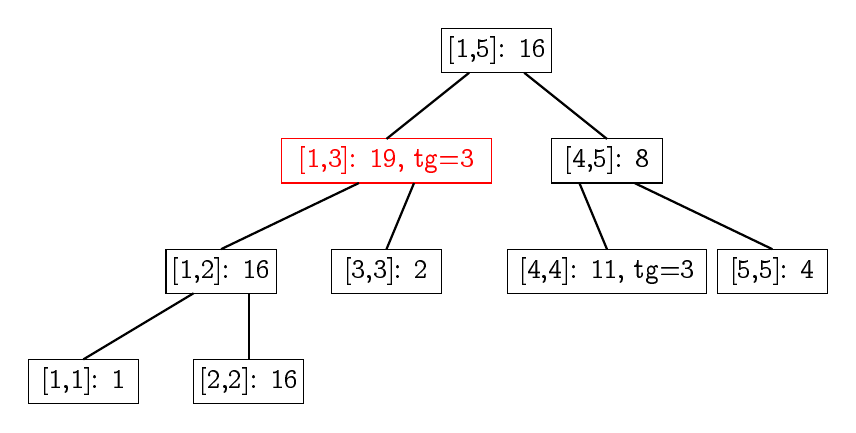
\begin{tikzpicture}[scale=0.7]
          \draw [black] (-1,7.9) rectangle (1,7.1) node [black, midway] {[1,5]: 16}; % Draws a rectangle

          \draw [red] (-3.9,5.9) rectangle (-0.1,5.1) node [red,midway] {[1,3]: 19, tg=3}; % Draws a rectangle
          \draw [black] (1,5.9) rectangle (3,5.1) node [black,midway] {[4,5]: 8}; % Draws a rectangle

          \draw [black] (-6,3.9) rectangle (-4,3.1) node [black,midway] {[1,2]: 16}; % Draws a rectangle
          \draw [black] (-3,3.9) rectangle (-1,3.1) node [black,midway] {[3,3]: 2}; % Draws a rectangle
          \draw [black] (0.2,3.9) rectangle (3.8,3.1) node [black,midway] {[4,4]: 11, tg=3}; % Draws a rectangle
          \draw [black] (4,3.9) rectangle (6,3.1) node [black,midway] {[5,5]: 4}; % Draws a rectangle

          \draw [black] (-8.5,1.9) rectangle (-6.5,1.1) node [black,midway] {[1,1]: 1}; % Draws a rectangle
          \draw [black] (-5.5,1.9) rectangle (-3.5,1.1) node [black,midway] {[2,2]: 16}; % Draws a rectangle

          \draw [thick] (-0.5,7.1) to (-2,5.9);
          \draw [thick] (0.5,7.1) to (2,5.9);

          \draw [thick] (-2.5,5.1) to (-5,3.9);
          \draw [thick] (-1.5,5.1) to (-2,3.9);

          \draw [thick] (1.5,5.1) to (2,3.9);
          \draw [thick] (2.5,5.1) to (5,3.9);

          \draw [thick] (-5.5,3.1) to (-7.5,1.9);
          \draw [thick] (-4.5,3.1) to (-4.5,1.9);
          % \draw [thick] (-2,2) % Draws a line
          % to [out=10,in=190] (2,2)
          % to [out=10,in=90] (6,0) 
          % to [out=-90,in=30] (-2,-2);    
        \end{tikzpicture}
      \end{figure}
  \end{itemize}
\end{frame}

\begin{frame}[fragile]{\btitle{懶人標記}}
  \begin{itemize}
    \item $a = [1, 16, 2, 8, 4]$,並把 $[1, 4]$ 加上 $3$,詢問 $[3, 3]$ 的最大值
    \item 把 tag 往下推?其實就是告訴左右孩子底下所有元素必須要加上 $3$
      \begin{figure}
        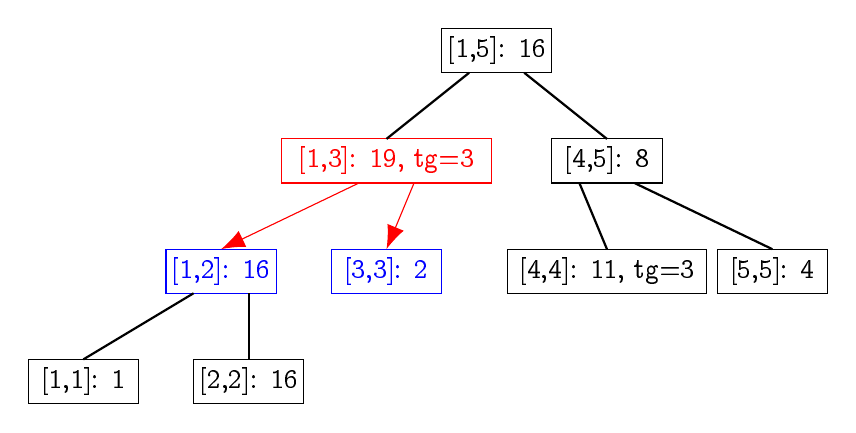
\begin{tikzpicture}[scale=0.7]
          \draw [black] (-1,7.9) rectangle (1,7.1) node [black, midway] {[1,5]: 16}; % Draws a rectangle

          \draw [red] (-3.9,5.9) rectangle (-0.1,5.1) node [red,midway] {[1,3]: 19, tg=3}; % Draws a rectangle
          \draw [black] (1,5.9) rectangle (3,5.1) node [black,midway] {[4,5]: 8}; % Draws a rectangle

          \draw [blue] (-6,3.9) rectangle (-4,3.1) node [blue,midway] {[1,2]: 16}; % Draws a rectangle
          \draw [blue] (-3,3.9) rectangle (-1,3.1) node [blue,midway] {[3,3]: 2}; % Draws a rectangle
          \draw [black] (0.2,3.9) rectangle (3.8,3.1) node [black,midway] {[4,4]: 11, tg=3}; % Draws a rectangle
          \draw [black] (4,3.9) rectangle (6,3.1) node [black,midway] {[5,5]: 4}; % Draws a rectangle

          \draw [black] (-8.5,1.9) rectangle (-6.5,1.1) node [black,midway] {[1,1]: 1}; % Draws a rectangle
          \draw [black] (-5.5,1.9) rectangle (-3.5,1.1) node [black,midway] {[2,2]: 16}; % Draws a rectangle

          \draw [thick] (-0.5,7.1) to (-2,5.9);
          \draw [thick] (0.5,7.1) to (2,5.9);

          \draw [red, arrows=-{Latex[length=3mm]}] (-2.5,5.1) -- (-5,3.9);
          \draw [red, arrows=-{Latex[length=3mm]}] (-1.5,5.1) -- (-2,3.9);

          \draw [thick] (1.5,5.1) to (2,3.9);
          \draw [thick] (2.5,5.1) to (5,3.9);

          \draw [thick] (-5.5,3.1) to (-7.5,1.9);
          \draw [thick] (-4.5,3.1) to (-4.5,1.9);
          % \draw [thick] (-2,2) % Draws a line
          % to [out=10,in=190] (2,2)
          % to [out=10,in=90] (6,0) 
          % to [out=-90,in=30] (-2,-2);    
        \end{tikzpicture}
      \end{figure}
  \end{itemize}
\end{frame}

\begin{frame}[fragile]{\btitle{懶人標記}}
  \begin{itemize}
    \item $a = [1, 16, 2, 8, 4]$,並把 $[1, 4]$ 加上 $3$,詢問 $[3, 3]$ 的最大值
    \item 把 tag 資訊丟給左右子樹,並且更新左右子樹的答案
      \begin{figure}
        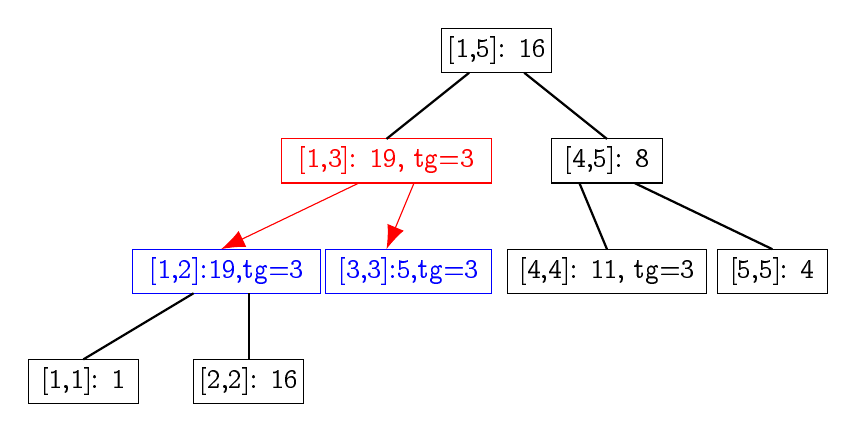
\begin{tikzpicture}[scale=0.7]
          \draw [black] (-1,7.9) rectangle (1,7.1) node [black, midway] {[1,5]: 16}; % Draws a rectangle

          \draw [red] (-3.9,5.9) rectangle (-0.1,5.1) node [red,midway] {[1,3]: 19, tg=3}; % Draws a rectangle
          \draw [black] (1,5.9) rectangle (3,5.1) node [black,midway] {[4,5]: 8}; % Draws a rectangle

          \draw [blue] (-6.6,3.9) rectangle (-3.2,3.1) node [blue,midway] {[1,2]:19,tg=3}; % Draws a rectangle
          \draw [blue] (-3.1,3.9) rectangle (-0.1,3.1) node [blue,midway] {[3,3]:5,tg=3}; % Draws a rectangle
          \draw [black] (0.2,3.9) rectangle (3.8,3.1) node [black,midway] {[4,4]: 11, tg=3}; % Draws a rectangle
          \draw [black] (4,3.9) rectangle (6,3.1) node [black,midway] {[5,5]: 4}; % Draws a rectangle

          \draw [black] (-8.5,1.9) rectangle (-6.5,1.1) node [black,midway] {[1,1]: 1}; % Draws a rectangle
          \draw [black] (-5.5,1.9) rectangle (-3.5,1.1) node [black,midway] {[2,2]: 16}; % Draws a rectangle

          \draw [thick] (-0.5,7.1) to (-2,5.9);
          \draw [thick] (0.5,7.1) to (2,5.9);

          \draw [red, arrows=-{Latex[length=3mm]}] (-2.5,5.1) -- (-5,3.9);
          \draw [red, arrows=-{Latex[length=3mm]}] (-1.5,5.1) -- (-2,3.9);

          \draw [thick] (1.5,5.1) to (2,3.9);
          \draw [thick] (2.5,5.1) to (5,3.9);

          \draw [thick] (-5.5,3.1) to (-7.5,1.9);
          \draw [thick] (-4.5,3.1) to (-4.5,1.9);
          % \draw [thick] (-2,2) % Draws a line
          % to [out=10,in=190] (2,2)
          % to [out=10,in=90] (6,0) 
          % to [out=-90,in=30] (-2,-2);    
        \end{tikzpicture}
      \end{figure}
  \end{itemize}
\end{frame}

\begin{frame}[fragile]{\btitle{懶人標記}}
  \begin{itemize}
    \item $a = [1, 16, 2, 8, 4]$,並把 $[1, 4]$ 加上 $3$,詢問 $[3, 3]$ 的最大值
    \item 原本的 tag 功成身退!
      \begin{figure}
        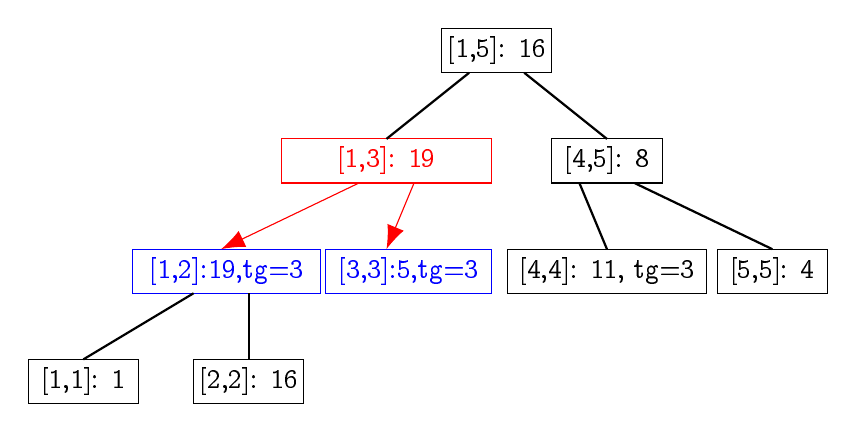
\begin{tikzpicture}[scale=0.7]
          \draw [black] (-1,7.9) rectangle (1,7.1) node [black, midway] {[1,5]: 16}; % Draws a rectangle

          \draw [red] (-3.9,5.9) rectangle (-0.1,5.1) node [red,midway] {[1,3]: 19}; % Draws a rectangle
          \draw [black] (1,5.9) rectangle (3,5.1) node [black,midway] {[4,5]: 8}; % Draws a rectangle

          \draw [blue] (-6.6,3.9) rectangle (-3.2,3.1) node [blue,midway] {[1,2]:19,tg=3}; % Draws a rectangle
          \draw [blue] (-3.1,3.9) rectangle (-0.1,3.1) node [blue,midway] {[3,3]:5,tg=3}; % Draws a rectangle
          \draw [black] (0.2,3.9) rectangle (3.8,3.1) node [black,midway] {[4,4]: 11, tg=3}; % Draws a rectangle
          \draw [black] (4,3.9) rectangle (6,3.1) node [black,midway] {[5,5]: 4}; % Draws a rectangle

          \draw [black] (-8.5,1.9) rectangle (-6.5,1.1) node [black,midway] {[1,1]: 1}; % Draws a rectangle
          \draw [black] (-5.5,1.9) rectangle (-3.5,1.1) node [black,midway] {[2,2]: 16}; % Draws a rectangle

          \draw [thick] (-0.5,7.1) to (-2,5.9);
          \draw [thick] (0.5,7.1) to (2,5.9);

          \draw [red, arrows=-{Latex[length=3mm]}] (-2.5,5.1) -- (-5,3.9);
          \draw [red, arrows=-{Latex[length=3mm]}] (-1.5,5.1) -- (-2,3.9);

          \draw [thick] (1.5,5.1) to (2,3.9);
          \draw [thick] (2.5,5.1) to (5,3.9);

          \draw [thick] (-5.5,3.1) to (-7.5,1.9);
          \draw [thick] (-4.5,3.1) to (-4.5,1.9);
          % \draw [thick] (-2,2) % Draws a line
          % to [out=10,in=190] (2,2)
          % to [out=10,in=90] (6,0) 
          % to [out=-90,in=30] (-2,-2);    
        \end{tikzpicture}
      \end{figure}
  \end{itemize}
\end{frame}

\begin{frame}[fragile]{\btitle{懶人標記}}
  \begin{itemize}
    \item 具體來說,之後某次區間修改或查詢而\textbf{造訪到某個節點時,我們才將這個節點的「標記」往下推},把標記的資訊傳給小孩
    \item 推標記的複雜度是 $O(1)$,不影響原本的複雜度!
    \item 因為是只在必要的時候更新標記,因此這個技巧又被稱為\textbf{懶人標記}
    \item 我們常把推標記的函數叫做 \texttt{push();}
    \item 直接來看程式碼吧~
  \end{itemize}
\end{frame}

\begin{frame}[fragile]{\btitle{懶人標記}}
  \begin{minted}[breaklines]{cpp}
    struct Node {
      Node *lc, *rc;
      int mx, tag; // tag 左右子樹整個子樹需要加上的數值
      void pull() { mx = max(lc->mx, rc->mx); }
    } *root = nullptr;
  \end{minted}
\end{frame}

\begin{frame}[fragile]{\btitle{懶人標記}}
  \begin{minted}[breaklines]{cpp}
    void push(Node *nd, int l, int r) {
      // 把 nd 的 tag 往左右子樹推
      if (l == r) nd->tag = 0;
      if (!nd->tag) return;
      nd->lc->tag += nd->tag; // 左子樹的 tag 跟 nd 的 tag 合併,這題 tag 是加上數值,因此直接加起來就可以
      nd->lc->mx  += nd->tag; // 左子樹的最大值加上 nd 的 tag
      nd->rc->tag += nd->tag;
      nd->rc->mx  += nd->tag;
      nd->tag = 0; // 清空 tag
    }
  \end{minted}
\end{frame}

\begin{frame}[fragile]{\btitle{懶人標記}}
  \begin{minted}[breaklines]{cpp}
    void modify(Node *nd, int ql, int qr, int d, int l, int r) {
      if (r < ql || l > qr)
        return;
      if (ql <= l && r <= qr) {
        nd->mx += d;  // 當前前點的所有數字加上 d,最大值也需要加上 d
        nd->tag += d; // 告訴左右子樹,最大值需要加上 d
        return;
      }
      push(nd, l, r); // 需要拜訪子樹的時候,把當前點的 tag 往下推
      int m = (l + r) / 2;
      modify(nd->lc, ql, qr, d, l, m);
      modify(nd->rc, ql, qr, d, m + 1, r);
      nd->pull();
    }
  \end{minted}
\end{frame}

\begin{frame}[fragile]{\btitle{懶人標記}}
  \begin{minted}[breaklines]{cpp}
    int query(Node *nd, int ql, int qr, int l, int r) {
      if (r < ql || l > qr)
        return 0;
      if (ql <= l && r <= qr)
        return nd->mx;
      push(nd, l, r); // 需要拜訪子樹的時候,把當前點的 tag 往下推
      int m = (l + r) / 2;
      return max(query(nd->lc, ql, qr, l, m), query(nd->rc, ql, qr, m + 1, r));
    }
  \end{minted}
\end{frame}

\begin{frame}[fragile]{\btitle{懶人標記}}
  \begin{itemize}
    \item 使用時機?
    \item 標記必須要可以合併、並且能夠快速的由「標記」所儲存的資訊推出這個節點的資訊應該被修改成什麼
    \item 有的時候順序很重要!
    \item 常見出現時機:區間加值區間求和、區間加值區間取 max、區間加值區間乘值區間求和......等等
    \item 不知道大家有沒有發現,\texttt{push()} 跟 \texttt{pull()} 好像會成對出現!
    \item 課外閱讀:有一種標記的方式叫「永久化標記」,這種標記就會直接把懶標固定在節點上,但詢問的時候就要多處理一些東西
  \end{itemize}
\end{frame}

\begin{frame}[fragile]{\btitle{copy on write 線段樹}}
  \begin{itemize}
    \item 又稱動態開點線段樹
    \item 需要使用的時候再把節點開出來!
    \item 直接來看例題:
    \begin{problem}[二維區間求和]
      給一 $N \times N(N \leq 10^9)$ 二維平面初始所有值都是零,$Q(Q \leq 10^5)$ 筆操作,操作包含兩種:
      \begin{itemize}
        \item \texttt{add x y d}: 將座標 $(x,y)$ 的元素加上 d
        \item \texttt{query x1 y1 x2 y2}: 詢問所有 $(x,y)$ 滿足 $x1 \leq x \leq x2$ 且 $y1 \leq y \leq y2$ 的總和。
      \end{itemize}
    \end{problem}
  \end{itemize}
\end{frame}

\begin{frame}[fragile]{\btitle{copy on write 線段樹}}
  \begin{itemize}
    \item 從題目的操作可以得知,最多只會有 $10^5$ 個座標有值
    \item 若是定義在一維座標上,我們可以利用\textbf{離散化}的技巧依然用我們前面介紹的線段樹解決
  \end{itemize}
\end{frame}

\begin{frame}[fragile]{\btitle{copy on write 線段樹}}
  \begin{itemize}    
    \item 然而,我們現在要處理的是二維座標
    \item 試著用線段樹套線段樹的方式吧!
    \item 等等,什麼是線段樹套線段樹?
  \end{itemize}
\end{frame}

\begin{frame}[fragile]{\btitle{copy on write 線段樹}}
  \begin{itemize}    
    \item 對 $x$ 軸開一個線段樹,$x$ 軸相關的節點的內容是對 $y$ 軸的線段樹!
      \begin{figure}
        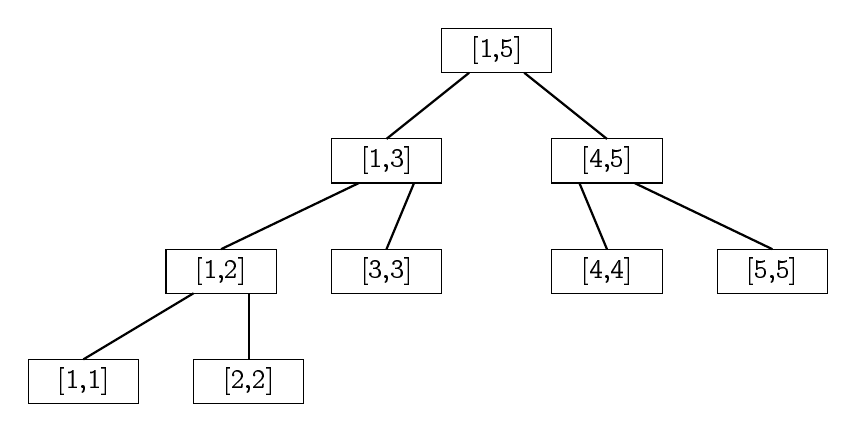
\begin{tikzpicture}[scale=0.7]
          \draw [black] (-1,7.9) rectangle (1,7.1) node [black, midway] {[1,5]}; % Draws a rectangle

          \draw [black] (-3,5.9) rectangle (-1,5.1) node [black,midway] {[1,3]}; % Draws a rectangle
          \draw [black] (1,5.9) rectangle (3,5.1) node [black,midway] {[4,5]}; % Draws a rectangle

          \draw [black] (-6,3.9) rectangle (-4,3.1) node [black,midway] {[1,2]}; % Draws a rectangle
          \draw [black] (-3,3.9) rectangle (-1,3.1) node [black,midway] {[3,3]}; % Draws a rectangle
          \draw [black] (1,3.9) rectangle (3,3.1) node [black,midway] {[4,4]}; % Draws a rectangle
          \draw [black] (4,3.9) rectangle (6,3.1) node [black,midway] {[5,5]}; % Draws a rectangle

          \draw [black] (-8.5,1.9) rectangle (-6.5,1.1) node [black,midway] {[1,1]}; % Draws a rectangle
          \draw [black] (-5.5,1.9) rectangle (-3.5,1.1) node [black,midway] {[2,2]}; % Draws a rectangle

          \draw [thick] (-0.5,7.1) to (-2,5.9);
          \draw [thick] (0.5,7.1) to (2,5.9);

          \draw [thick] (-2.5,5.1) to (-5,3.9);
          \draw [thick] (-1.5,5.1) to (-2,3.9);

          \draw [thick] (1.5,5.1) to (2,3.9);
          \draw [thick] (2.5,5.1) to (5,3.9);

          \draw [thick] (-5.5,3.1) to (-7.5,1.9);
          \draw [thick] (-4.5,3.1) to (-4.5,1.9);
          % \draw [thick] (-2,2) % Draws a line
          % to [out=10,in=190] (2,2)
          % to [out=10,in=90] (6,0) 
          % to [out=-90,in=30] (-2,-2);
        \end{tikzpicture}
      \end{figure}
    \item 比如說,$[1, 3]$ 這個節點存一個 $y$ 軸資訊的線段樹,$y$ 軸線段樹的 $[4, 5]$ 就是存 $[1..3, 4..5]$ 的總和!
  \end{itemize}
\end{frame}

\begin{frame}[fragile]{\btitle{copy on write 線段樹}}
  \begin{itemize}    
    \item 雖然做完離散化,還是 $O(Q^2)$ 的空間
    \item 但,最多只有 $Q$ 個座標有值,因此,最多只有 $O(Q \lg^2 N)$ 個節點有值!只要能只記錄這些節點便勝利了
    \begin{itemize}
      \item 在 $x$ 軸的世界中會經過 $O(\log N)$ 個節點
      \item 每個節點的線段樹需要經過 $O(\log N)$ 個 $y$ 軸節點
    \end{itemize}
    \item 來看 code 吧!
  \end{itemize}
\end{frame}

\begin{frame}[fragile]{\btitle{copy on write 線段樹}}
  \begin{minted}[breaklines]{cpp}
    struct Node2 { // 第二個維度的線段樹節點
      int val;
      Node2 *lc, *rc;
      Node2() {
        val = 0;
        lc = rc = NULL;
      }
    };
    struct Node1 { // 第一個維度的線段樹節點
      Node1 *lc, *rc;
      Node2 *c;
      Node1() {
        c = NULL;
        lc = rc = NULL;
      }
    };
  \end{minted}
\end{frame}

\begin{frame}[fragile]{\btitle{copy on write 線段樹}}
  \begin{minted}[breaklines]{cpp}
    int Val2(Node2 *node) { return node ? node->val : 0; }
    void pull2(Node2 *node) { node->val = Val2(node->lc) + Val2(node->rc); }
  \end{minted}
\end{frame}

\begin{frame}[fragile]{\btitle{copy on write 線段樹}}
  \begin{minted}[breaklines]{cpp}
    void modify2(Node2 *node, int Y1, int Y2, int qy, int d) {
      if (Y1 == Y2) {
        node->val += d;
        return;
      }
      int mid = (Y1 + Y2) >> 1;
      if (qy <= mid) {
        if (!node->lc) node->lc = new Node2(); // 有需要再開新的 y 軸點
        modify2(node->lc, Y1, mid, qy, d);
      } else {
        if (!node->rc) node->rc = new Node2();
        modify2(node->rc, mid + 1, Y2, qy, d);
      }
      pull2(node);
    }
  \end{minted}
\end{frame}

\begin{frame}[fragile]{\btitle{copy on write 線段樹}}
  \begin{minted}[breaklines]{cpp}
    void modify1(Node1 *node, int X1, int X2, int qx, int qy, int d) {
      if (!node->c) node->c = new Node2(); // 有需要再開新的 y 軸點
      modify2(node->c, 1, n, qy, d);
      if (X1 == X2) {
        return;
      }
      int mid = (X1 + X2) >> 1;
      if (qx <= mid) {
        if (!node->lc) node->lc = new Node1(); // 有需要再開新的 x 軸點
        modify1(node->lc, X1, mid, qx, qy, d);
      } else {
        if (!node->rc) node->rc = new Node1();
        modify1(node->rc, mid + 1, X2, qx, qy, d);
      }
    }
  \end{minted}
\end{frame}

\begin{frame}[fragile]{\btitle{copy on write 線段樹}}
  \begin{minted}[breaklines]{cpp}
    int query2(Node2 *node, int Y1, int Y2, int qy1, int qy2) {
      if (qy1 > Y2 || qy2 < Y1)
        return 0;
      if (!node)
        return 0; // no data!
      if (qy1 <= Y1 && Y2 <= qy2)
        return node->val;
      int mid = (Y1 + Y2) >> 1;
      return query2(node->lc, Y1, mid, qy1, qy2) +
             query2(node->rc, mid + 1, Y2, qy1, qy2);
    }
  \end{minted}
\end{frame}

\begin{frame}[fragile]{\btitle{copy on write 線段樹}}
  \begin{minted}[breaklines]{cpp}
    int query1(Node1 *node, int X1, int X2, int qx1, int qx2, int qy1, int qy2) {
      if (qx1 > X2 || qx2 < X1)
        return 0;
      if (!node)
        return 0; // no data!
      if (qx1 <= X1 && X2 <= qx2)
        return query2(node->c, 1, n, qy1, qy2);
      int mid = (X1 + X2) >> 1;
      return query1(node->lc, X1, mid, qx1, qx2, qy1, qy2) +
             query1(node->rc, mid + 1, X2, qx1, qx2, qy1, qy2);
    }
  \end{minted}
\end{frame}

\begin{frame}[fragile]{\btitle{持久化線段樹}}
  \begin{itemize}
    \item 修改後依舊保有歷史版本的資料結構
    \item 直接來看例題:
    \begin{problem}[歷史版本和]
      給定一個長度 $N$ 的序列以及 $M$ 個單點修改,接下來有 $Q$ 次詢問,每次詢問會問你在第 $m$ 次修改後,區間 $[l, r]$ 的總和是多少。
      強制在線。
      
      \begin{itemize}
          \item
              $N, Q \leq 10^5$
      \end{itemize}
    \end{problem}
  \end{itemize}
\end{frame}

\begin{frame}[fragile]{\btitle{持久化線段樹}}
  \begin{itemize}
    \item 我會!
    \item 每個版本各開一個線段樹就好啦~
    \item 總共需要 $O(N)$ 個版本,每個版本 $O(N)$ 個點,總共 $O(N^2)$ 個點,TLE!
    \item 怎麼辦 OuO
  \end{itemize}
\end{frame}

\begin{frame}[fragile]{\btitle{持久化線段樹}}
  \begin{itemize}
    \item 努力觀察一下:每次修改都只會動到 $O(\log N)$ 個節點
      \begin{itemize}
        \item 這些節點其實就是單點修改碰到的那些點
      \end{itemize}
    \item 那麼我們為何不能用 $O(\log N)$ 的空間來儲存兩個版本之間的差距呢?
  \end{itemize}
\end{frame}

\begin{frame}[fragile]{\btitle{持久化線段樹}}
  \begin{itemize}
    \item 努力觀察一下:每次修改都只會動到 $O(\log N)$ 個節點
    \item 那麼我們為何不能用 $O(\log N)$ 的空間來儲存兩個版本之間的差距呢?
    \item 具體來說,我們每次想要更新一個節點的值時,會開出一個新節點儲存修改之後的資訊(不要看下面那張圖的 $e$ 點)
  \end{itemize}
  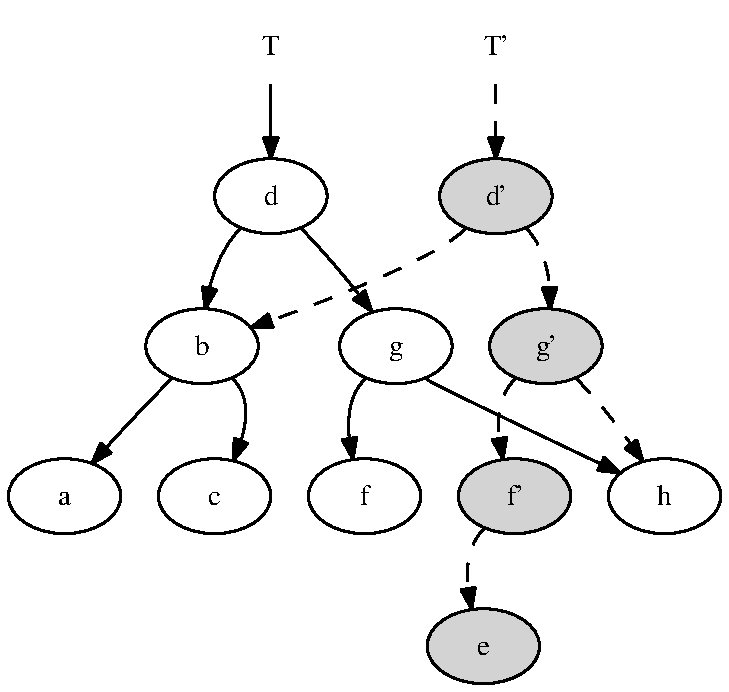
\includegraphics[height=4.5cm]{figures/persistent-tree.pdf}
\end{frame}

\begin{frame}[fragile]{\btitle{持久化線段樹}}
  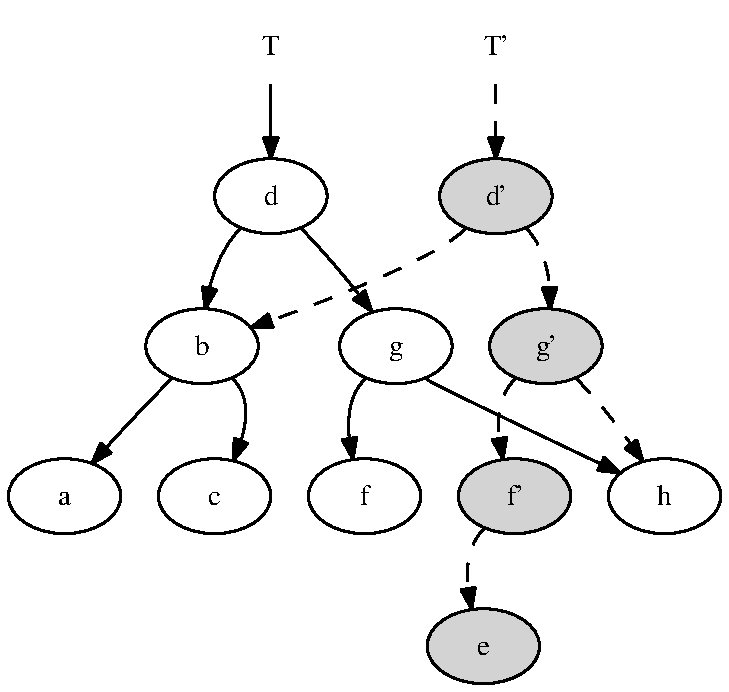
\includegraphics[height=4.5cm]{figures/persistent-tree.pdf}
  \begin{itemize}
    \item 所以,每當需要一個新的版本的時候
    \item 先把舊版本根節點重新複製一遍到新版本的根節點上
    \item 每當要進入某個點修改時,先把該節點複製一份到新版本上
    \item 遞迴修改
    \item 修改結束後,因為新節點的子樹有變動,呼叫新節點的 \texttt{pull()}
  \end{itemize}
\end{frame}

\begin{frame}[fragile]{\btitle{持久化線段樹}}
  \begin{minted}[breaklines]{cpp}
    // get a copy of node
    Node *getNode(Node *node) {
      Node *tnode = new Node();
      tnode->val = node->val;
      tnode->lc = node->lc;
      tnode->rc = node->rc;
      return tnode;
    }
  \end{minted}
\end{frame}

\begin{frame}[fragile]{\btitle{持久化線段樹}}
  \begin{minted}[breaklines]{cpp}
    void modify(Node *node, Node *newNode, int L, int R, int i, int d) {
      if (L == R) {
        newNode->val += d;
        return;
      }
      int mid = (L + R) >> 1;
      if (i <= mid) {
        newNode->lc = getNode(node->lc);
        modify(node->lc, newNode->lc, L, mid, i, d);
      } else {
        newNode->rc = getNode(node->rc);
        modify(node->rc, newNode->rc, mid + 1, R, i, d);
      }
      newNode->pull();
    }
  \end{minted}
\end{frame}

\begin{frame}[fragile]{\btitle{持久化線段樹}}
  \begin{itemize}
    \item 很常運用在序列上!
    \item 常見建立的版本時機是:給定一個長度為 $N$ 的序列,建立 $N$ 個版本,第 $i$ 個版本維護第 $i$ 個位置的前綴(或者是後綴)的資訊
  \end{itemize}
\end{frame}

\begin{frame}[fragile]{\btitle{STL in 線段樹}}
  \begin{itemize}
    \item 線段樹的節點可以塞各式各樣的東西喔!
    \begin{problem}[二維區間求和]
      有 $n$ 個目標物,每個目標物都是一個水平線段 $[s, t]$ 或是只含一點($s = t$ 的情形),並且有各自的分數 $w$,所有目標物的高度($y$ 值)均大於 $0$ 且互不相同(輸入按照 $y$ 座標由大到小排序)。
      現在依序發射了 $m$ 發砲彈,第 $i$ 次會從 $x$ 軸上的整數點 $x_i$ 往上垂直發射砲彈,路線上第一個碰到的目標物就是擊中的目標,射中目標後砲彈與目標物一起消失,不會穿透。如果沒有擊中任何目標物,則該次射擊分數為 0。請輸出每次有擊中的目標物的分數總和。
      \begin{itemize}
        \item $n, m \leq 5 \times 10^5$
        \item $s,t,x_i \leq 10^6$
      \end{itemize}
    \end{problem}
  \end{itemize}
\end{frame}

\begin{frame}[fragile]{\btitle{STL in 線段樹}}
  \begin{itemize}
    \item 在線段樹的每個節點當中,我們可以儲存一個 set
    \item set 裡面放一些完全包含這個節點對應的區間的水平線段
    \item 我們可以做 $n$ 次的區間修改,在對應的節點裡面的 set 插入這個水平線段的 $y$ 座標
    \item 對於每次的單點詢問,我們查看對應的葉節點到根的這條路徑上, $y$ 座標最小的水平線段是哪一個
    \item 當知道哪個水平線段要被刪除之後,可以做一次區間修改,並且在對應的節點裡面的 set 刪除這個水平線段的 $y$ 座標
    \item 因為每次都會造訪 $O(\log n)$ 個節點,而 std::set 插入、刪除的複雜度都是 $O(\log n)$,因此總共的複雜度會是 $((n+m)\log ^2 n)$,空間複雜度則是 $O(n\log n)$
  \end{itemize}
\end{frame}

\begin{frame}[fragile]{\btitle{STL in 線段樹}}
  \begin{itemize}
    \item 事實上我們可以用一個 std::vector(或是 stack)來維護這樣的插入與刪除,因為所有刪除操作都在插入之後,如此時間複雜度可以減少一個 $\log$
    \item 注意 STL 的 stack 內部預設是 deque,而空的 deque 佔的空間很多,因此在這種嵌套的資料結構特別要小心
  \end{itemize}
\end{frame}

\begin{frame}[fragile]{\btitle{區間查詢與修改的對偶}}
  \begin{itemize}
    \item 直接來看例題!
    \begin{problem}[區間取 max、單點查詢]
      有一長度為 $N$ 的序列 $a_1,a_2,\dots,a_N$,一開始全部為 $0$。接下來有 $M$ 個操作,每個操作形如 $l, r, v$ ,表示對於所有 $l \leq i \leq r$,$a_i := \max(a_i, v)$。
      請你分別輸出 $a_1,a_2,\dots, a_N$ 最後的值是多少。

      \begin{itemize}
          \item
              $N \leq 2\times 10^5$
          \item
              $M \leq 5\times 10^6$
      \end{itemize}
    \end{problem}
  \end{itemize}
\end{frame}

\begin{frame}[fragile]{\btitle{區間查詢與修改的對偶}}
  \begin{itemize}
    \item 相信在前面學過懶人標記後,大家已經知道如何用線段樹與懶人標記解決這個問題了
    \item 然而這樣做的複雜度是 $O(N+M\log N)$,很有可能無法在時限內通過
    \item 為什麼呢?因為詢問的數量太多了
    \item 但相對的,\textbf{修改沒那麼多},並且\textbf{我們可以一次處理所有修改}
    \item 有什麼資料結構是支援快速查詢,且可以利用離線的性質呢?
    \item Sparse Table!
  \end{itemize}
\end{frame}

\begin{frame}[fragile]{\btitle{區間查詢與修改的對偶}}
  \begin{itemize}
    \item 在 Sparse Table 中是把一個區間查詢拆成兩個部份重疊的區間查詢,並且兩個區間的長度為 2 的冪次
    \item 那麼我們也可以把區間修改拆成兩個長度為 2 的冪次的區間,並紀錄所有 $g(i, j)$ 表示 $[i, i+2^j)$ 整個區間要跟多少取 max
    \item 最後再一次花 $O(N\log N)$ DP 便能得到每個單獨的位置是多少
      \begin{itemize}
        \item 類似 sparse table 預處理的方式
        \item 只是這次是從上面往下推(sparse table 預處理是下面往上推)
      \end{itemize}
    \item 因此總複雜度為 $O(N\log N + M)$,空間複雜度是 $O(N\log N)$
  \end{itemize}
\end{frame}

\begin{frame}[fragile]{\btitle{區間查詢與修改的對偶}}
  \begin{minted}[breaklines]{cpp}
    int st[maxlg][maxn];
    void chmax(int l, int r, int val) {
      // for i \in [l, r), a[i] = max(a[i], val)
      int lg = __lg(r - l);
      int len = 1 << lg;
      st[lg][l] = max(st[lg][l], val);
      st[lg][r - len] = max(st[lg][r - len], val);
    }
  \end{minted}
\end{frame}

\begin{frame}[fragile]{\btitle{區間查詢與修改的對偶}}
  \begin{minted}[breaklines]{cpp}
    void dp(int n) {
      for (int l = maxlg - 2; l >= 0; l--) {
        int len = 1 << l;
        for (int i = 0; i < n; i++) {
          st[l][i] = max(st[l][i], st[l + 1][i]);
          if (i + len < n)
            st[l][i + len] = max(st[l][i + len], st[l + 1][i]);
        }
      }
      // ans is st[0][i]
    }
  \end{minted}
\end{frame}

\begin{frame}[fragile]{\btitle{區間查詢與修改的對偶}}
  \begin{itemize}
    \item 網路上有一個類似的技巧被稱為 Dual Segment Tree,但比較侷限在線段樹而沒有其他推廣
    \item 事實上這個技巧除了 Sparse Table 外,分塊、樹上倍增法、線段樹都可以用到
    \item 值得注意的是線段樹一次 push 所有節點的懶標只需要 $O(N)$
      \begin{itemize}
        \item DFS 一次整棵樹就可以了!
      \end{itemize}
  \end{itemize}
\end{frame}

\begin{frame}[fragile]{\btitle{線段樹上的均攤}}
  \begin{itemize}
    \item 直接來看例題!
    \begin{problem}[區間取 max、單點查詢]
      給定一個長度 $N$ 的序列 $a_1,\dots,a_N$,接下來有 $Q$ 個操作:
      \begin{itemize}
          \item \(\texttt{A x v}\) 將 $a_x$ 改為 $v$。
          \item \(\texttt{D l r k}\) 對於所有 $l\leq i\leq r$,將 $a_i$ 改為 $\lfloor \frac{a_i}{k} \rfloor$。
          \item \(\texttt{S l r}\) 查詢區間 $[l, r]$ 的總和。
      \end{itemize}
      輸入的所有數字均為正整數。

      \begin{itemize}
          \item
              $N, Q \leq 10^5$
          \item
              $1 \leq a_i, v, k \leq 10^9$
      \end{itemize}
    \end{problem}
  \end{itemize}
\end{frame}

\begin{frame}[fragile]{\btitle{線段樹上的均攤}}
  \begin{itemize}
    \item 本題出現了一個非常神秘的操作:區間除法取下高斯
    \item 我們無法快速由分母推出整個區間的總和如何變化,要怎麼處理這樣的問題呢?
    \item 不是整個區間都是 $0$,就暴力 DFS 下去!
    \item 這樣是好的嗎...... (?)
    \item 亂寫一通就發現 AC 了,怎麼會這樣!
  \end{itemize}
\end{frame}

\begin{frame}[fragile]{\btitle{線段樹上的均攤}}
  \begin{itemize}
    \item 可以發現,每個數字被除了 $O(\log C)$ 次之後就會變成 $0$(當然,不包含 $k=1$ 的情況)
    \item 而每個數字每除一次又最多只會讓時間增加樹高的量級
    \item 至於單點修改也只會讓除的次數增加 $\log C$ 次
    \item 因此,總複雜度便是 $O((N+Q)\log N \log C)$
    \item 除了除法之外,區間開根號、區間取 $\log$ 都可以用類似的技巧喔!
  \end{itemize}
\end{frame}

\begin{frame}[fragile]{\btitle{搭配離線演算法}}
  \begin{itemize}
    \item 「離線回答的精髓」:可以事前知道所有詢問的所有參數,並且可以不按順序回答每個詢問
    \item 什麼意思?來看前面持久化線段樹例題的離線版本
    \item
      \begin{problem}[歷史版本和 -- offline]
        給定一個長度 $N$ 的序列以及 $M$ 個單點修改,接下來有 $Q$ 次詢問,每次詢問會問你在第 $m$ 次修改後,區間 $[l, r]$ 的總和是多少。
        
        \begin{itemize}
            \item
                $N, Q \leq 10^5$
        \end{itemize}
      \end{problem}
    \item 為什麼我不要乾脆一邊做修改、等到剛好第 $m$ 次修改之後再回答詢問就好了
    \item 而這個就是「離線回答的精髓」:可以事前知道所有詢問的所有參數,並且可以不按順序回答每個詢問
  \end{itemize}
\end{frame}

\begin{frame}[fragile]{\btitle{搭配離線演算法}}
  \begin{itemize}    
    \item 離線演算法大致上的套路都是把詢問和修改(原本的序列也可以當成是某種修改)一起按照某種順序排序
    \item 接著一邊處理修改一邊處理詢問
    \item 並把所有詢問的答案存下來後一次回答全部
    \item 事實上,許多問題「在線回答」與「離線回答」的難度相差很多,也有很多知名的演算法必須在離線的問題才能使用
    \item 來看例題吧!
  \end{itemize}
\end{frame}

\begin{frame}[fragile]{\btitle{搭配離線演算法}}
  \begin{itemize}
    \item 
      \begin{problem}[區間 mex]
        給定一個序列 $a_1,a_2,\dots,a_N$,接下來有 $Q$ 個詢問,每次會給定 $l, r$,請你回答 $\operatorname{mex}(a_l,a_{l+1},\dots,a_r)$。
        其中 $\operatorname{mex}$ 的定義是一個集合中最小未出現的非負整數。

        \begin{itemize}
            \item
                $N, Q \leq 2\times 10^5$
        \end{itemize}

        比如說,$\operatorname{mex}(1, 3) = 0$, $\operatorname{mex}(0, 1, 3) = 2$
      \end{problem}
    \item 題外話:這題可以用莫隊 + 值域分塊在 $O((N + Q)\sqrt{N})$ 做掉,不過不在這堂課的討論範疇(偷偷工商,可以看資芽 2021 年根號 inclass 的投影片喔)
    \item 好像不太清楚 \texttt{pull()} 要怎麼寫耶,怎麼辦?
    \item 先來考慮一個簡單一點的版本!
  \end{itemize}
\end{frame}

\begin{frame}[fragile]{\btitle{搭配離線演算法}}
  \begin{itemize}
    \item 
      \begin{problem}[區間 mex --- 簡化版]
        給定一個序列 $a_1,a_2,\dots,a_N$,接下來有 $Q$ 個詢問,每次會給定 $r$,請你回答 $\operatorname{mex}(a_1,a_{l+1},\dots,a_r)$。
        其中 $\operatorname{mex}$ 的定義是一個集合中最小未出現的非負整數。

        \begin{itemize}
            \item
                $N, Q \leq 2\times 10^5$
        \end{itemize}

        比如說,$\operatorname{mex}(1, 3) = 0$, $\operatorname{mex}(0, 1, 3) = 2$
      \end{problem}
    \item 現在左界通通變成 $1$ 了,但我們好像還不知道線段樹要怎麼維護?
    \item 在這之前中,線段樹的葉節點 $[i, i]$ 常常只用來維護 $a_i$ 相關的資訊,讓我們來跳脫這個框架! 
  \end{itemize}
\end{frame}

\begin{frame}[fragile]{\btitle{搭配離線演算法}}
  \begin{itemize}
    \item 
      \begin{problem}[區間 mex --- 簡化版]
        給定一個序列 $a_1,a_2,\dots,a_N$,接下來有 $Q$ 個詢問,每次會給定 $r$,請你回答 $\operatorname{mex}(a_1,a_{1+1},\dots,a_r)$。
        其中 $\operatorname{mex}$ 的定義是一個集合中最小未出現的非負整數。

        \begin{itemize}
            \item
                $N, Q \leq 2\times 10^5$
        \end{itemize}
      \end{problem}
    \item 想想看我們是怎麼做 \texttt{mex()} 運算的
    \item 假設現在在回答 $[1, r]$:從 $0, 1, \dots, N$ 開始一路往下看,看哪個數字最早沒出現在 $a_1$ 到 $a_r$ 中
    \item 也就是說,我們要關心「數值本身」的出現狀況(關心的本質),搞不好線段樹 $[i, i]$ 的葉節點要維護\textbf{數字 $i$ 相關的資訊} 
  \end{itemize}
\end{frame}

\begin{frame}[fragile]{\btitle{搭配離線演算法}}
  \begin{itemize}
    \item 
      \begin{problem}[區間 mex --- 簡化版]
        給定一個序列 $a_1,a_2,\dots,a_N$,接下來有 $Q$ 個詢問,每次會給定 $r$,請你回答 $\operatorname{mex}(a_1,a_{1+1},\dots,a_r)$。
        其中 $\operatorname{mex}$ 的定義是一個集合中最小未出現的非負整數。
      \end{problem}
    \item 回到原本的問題,要怎麼快速的判斷一個數字有沒有出現在 $a_1$ 到 $a_r$
    \item 觀察一:如果一個數字在序列出現很多次,我們可以\textbf{拿最左邊的點當這個數字代表},我們可以把這些數字單獨拿出來
    \item $[{\color{red} 2}, 2, {\color{red} 0}, {\color{red} 1}, 0]$
  \end{itemize}
\end{frame}

\begin{frame}[fragile]{\btitle{搭配離線演算法}}
  \begin{itemize}
    \item $[{\color{red} 2}, 2, {\color{red} 0}, {\color{red} 1}, 0]$
    \item 把紅色數字拿出來當作資訊用
    \item 數字 $0$ 最早出現在 $a_3$,數字 $1$ 最早出現在 $a_4$,數字 $2$ 最早出現在 $a_1$,數字 $3$ 最早出現在 $a_{N + 1}$(不存在)
      \begin{itemize}
        \item 在上面的例子中,$f(0) = 3, f(1) = 4, f(2) = 1, f(3) = N + 1$
      \end{itemize}
    \item 假設我們用 $f(i)$ 來存這個資訊:$f(i)$ 代表數字 $i$ 在 $a$ 序列中最早出現的位置
    \item 有上面的資訊之後,要怎麼判斷數字 $i$ 有沒有出現在 $a_1$ 到 $a_r$ 呢?
    \item \texttt{\textbf{f(i) <= r} ? "Yes" : "No"}
  \end{itemize}
\end{frame}

\begin{frame}[fragile]{\btitle{搭配離線演算法}}
  \begin{itemize}
    \item $[{\color{red} 2}, 2, {\color{red} 0}, {\color{red} 1}, 0]$
    \item 假設我們用 $f(i)$ 來存這個資訊:$f(i)$ 代表數字 $i$ 在 $a$ 序列中最早出現的位置
    \item 有上面的資訊之後,要怎麼判斷數字 $i$ 有沒有出現在 $a_1$ 到 $a_r$ 呢?
    \item \texttt{\textbf{f(i) <= r} ? "Yes" : "No"}
    \item 會判斷一個數字了,來回到原本的詢問:從 $0, 1, \dots, N$ 開始一路往下看,看哪個數字最早沒出現在 $a_1$ 到 $a_r$ 中
    \item \textbf{那其實就是找到最小的 $i$,滿足 $f(i) > r$}
    \item 二分搜尋!
  \end{itemize}
\end{frame}

\begin{frame}[fragile]{\btitle{搭配離線演算法}}
  \begin{itemize}
    \item $[{\color{red} 2}, 2, {\color{red} 0}, {\color{red} 1}, 0]$
    \item 假設我們用 $f(i)$ 來存這個資訊:$f(i)$ 代表數字 $i$ 在 $a$ 序列中最早出現的位置
    \item 原本的詢問就等價,\textbf{找到最小的 $i$,滿足 $f(i) > r$}
    \item 二分搜尋!
      \begin{minted}[breaklines]{cpp}
        int bs_l = -1, bs_r = n + 1;
        while (bs_r - bs_l > 1) {
          int mid = (bs_l + bs_r) >> 1;
          if (query_max(0, mid) > r) bs_r = mid;
          else bs_l = mid;
        }
        // answer stored in bs_r
      \end{minted}
    \item \texttt{query\_max(L, R)} 是詢問 $f(L)$ 到 $f(R)$ 的最大值,乍看之下可以用 Sparse Table 讓複雜度是 $O(\log N)$ 
  \end{itemize}
\end{frame}

\begin{frame}[fragile]{\btitle{搭配離線演算法}}
  \begin{itemize}
    \item 
      \begin{problem}[區間 mex --- 中階版]
        給定一個序列 $a_1,a_2,\dots,a_N$,接下來有 $Q$ 個詢問,每次會給定 $l, r$,請你回答 $\operatorname{mex}(a_l,a_{l+1},\dots,a_r)$ ,但題目保證 $l \in [1, 2]$。
        其中 $\operatorname{mex}$ 的定義是一個集合中最小未出現的非負整數。
      \end{problem}
    \item 在簡化版中,我們可以用二分搜處理所有 $l = 1$ 的狀況
    \item 那同樣的,我們就可以\textbf{把 $l = 1$ 跟 $l = 2$}的詢問分開,先處理所有 $l = 2$ 再處理所有 $l = 1$(個別二分搜)
    \item \textbf{但從 $l = 2$ 移動到 $l = 1$ 的過程中,我們需要把 $f(a_1) = 1$}
    \item 所以,維護 $f()$ 的資料結構要支援單點修改,\textbf{就不能用 Sparse Table,要用線段樹了}
  \end{itemize}
\end{frame}

\begin{frame}[fragile]{\btitle{搭配離線演算法}}
  \begin{itemize}
    \item 
      \begin{minted}[breaklines]{cpp}
        int bs_l = -1, bs_r = n + 1;
        while (bs_r - bs_l > 1) {
          int mid = (bs_l + bs_r) >> 1;
          if (query_max(0, mid) > r) bs_r = mid;
          else bs_l = mid;
        }
        // answer stored in bs_r
      \end{minted}
    \item 但是這樣,複雜度就變成 $O(\log^2 N)$,有沒有辦法維持一個 $\log$ 呢?
    \item 跟 BIT 的狀況類似,\textbf{我們可以在線段樹這個結構上面二分搜!}
    \item 直接看 code 吧~
  \end{itemize}
\end{frame}

\begin{frame}[fragile]{\btitle{搭配離線演算法}}
  \begin{minted}[breaklines]{cpp}
    int binsearch(int k, Node *now, int l, int r) {
      if (l == r)
        return l;
      int m = l + (r - l) / 2;
      if (now->l->mx > k) // 左邊的最大值 > k,代表答案在線段樹的左子樹這
        return binsearch(k, now->l, l, m);
      else
        return binsearch(k, now->r, m + 1, r);
    }
  \end{minted}
\end{frame}

\begin{frame}[fragile]{\btitle{搭配離線演算法}}
  \begin{itemize}
    \item 來推廣到整個題目吧!
    \item 我們由 $a_N$ 至 $a_1$ 的順序依序掃過原本的序列,並且將其加入某個資料結構
    \item 在掃到 $a_i$ 的時候,這個資料結構裡面儲存了包含順便處理左界為 $i$ 的詢問
    \item 定義 $f_j$ 表示數字 $j$ 在 $[i, N]$ 最前面出現的位置
    \item 那麼 $\operatorname{mex}(i, r)$ 就是最小的數字使得 $\max_{i \leq j \leq r}(f_j) > r$
    \item 所以,我們可以用一個線段樹維護 $f_j$ 的區間最大值,再搭配上二分搜,就能回答所有詢問了
    \item 二分搜可以直接在線段樹上二分搜,把複雜度壓到 $O((N+Q)\log N)$ 的複雜度
    \item 這種線段樹,位置 $i$ 是存關於數值 $i$ 的資訊,而不是序列第 $i$ 個位置的資訊,我們常稱為這是「值域線段樹」
  \end{itemize}
\end{frame}

\begin{frame}[fragile]{\btitle{區間查詢與修改的對偶}}
  \begin{minted}[breaklines]{cpp}
    struct Node {
      Node *l, *r;
      int mx;
      void pull() { mx = max(l->mx, r->mx); }
    };
  \end{minted}
\end{frame}

\begin{frame}[fragile]{\btitle{區間查詢與修改的對偶}}
  \begin{minted}[breaklines]{cpp}
    for (int i = 0; i < Q; i++) {
      queries.emplace_back(l, r, i);
    }
    sort(queries.begin(), queries.end(), greater<>());
    root = build(0, N);
    int it = 0;
    for (int i = N; i >= 1; i--) {
      if (a[i] <= N)
        edit(a[i], i, root, 0, N);
      while (it < queries.size() && get<0>(queries[it]) == i) {
        auto [l, r, qid] = queries[it++];
        ans[qid] = binsearch(r, root, 0, N);
      }
    }
  \end{minted}
\end{frame}

\begin{frame}[fragile]{\btitle{資料結構經典題}}
  \begin{itemize}
    \item 直接來看例題!
    \begin{problem}[K-th Number]
      給長度 $N$ 的序列 $a$,及 $Q$ 筆詢問。
      每筆詢問給 $i,j,k$,求 $[i,j]$ 區間中第 $k$ 小數。
      (即把 $[i,j]$ 區間由小到大排序後,第 $k$ 個數)
      
      \begin{itemize}
          \item
              $1 \leq N \leq 10^5$
          \item
              $1 \leq Q \leq 10^5$
          \item
              $1 \leq i \leq j \leq N, k\leq(j-i+1)$
      \end{itemize}
    \end{problem}
  \end{itemize}
\end{frame}

\begin{frame}[fragile]{\btitle{資料結構經典題}}
  \begin{itemize}
    \item 這題如果允許離線的話,可以使用整體二分在 $O((Q + N) \log N)$ 或 $O((Q + N) \log^2 N)$ 內做完,詳細部份可以參考這本講義分治這個單元
    \item 我們可以考慮使用值域線段樹來解決這個問題,線段樹每個位置存這個數字出現了幾次
    \item 而要找到第 $K$ 小,就可以直接在值域線段樹上面二分搜就好(作法類似 BIT 第 K 小的作法,加上在前面區間 mex 操作在線段樹上二分搜的技巧)
  \end{itemize}
\end{frame}

\begin{frame}[fragile]{\btitle{資料結構經典題}}
  \begin{itemize}
    \item 而現在,我們可以把這樣的值域線段樹外面套上一層「持久化」
    \item 我們開一個 $N$ 個版本的值域線段樹,第 $i$ 個版本存 $a_1$ 到 $a_i$ 項中每個數字出現過的次數
    \item 在進行詢問的時候,就可以利用「第 $r$ 個版本」扣掉「第 $l - 1$ 個版本」,來獲得區間 $[l, r]$ 的值域的狀況,進而在上面二分搜!
    \item 直接來看講義的程式碼吧~
  \end{itemize}
\end{frame}

\end{document}


\documentclass[standalone]{beamer}

\begin{document}
\section{樹堆}

\begin{frame}[fragile]{樹堆}
  \begin{itemize}
    \item Treap
    \item Tree + Heap
    \item 樹堆是一種二元樹,是 Binary Search Tree + Heap 的綜合題
    \item 節點有兩個值:pri 跟 key,分別滿足\textbf{二元搜尋樹}的性質跟\textbf{堆}的性質
  \end{itemize}
\end{frame}

\begin{frame}[fragile]{樹堆}
  \begin{itemize}
    \item 樹性質:
    \begin{itemize}
      \item 左子樹的 key 都小於根節點的 key
      \item 左子樹的 key 都大於根節點的 key
      \item 左右子樹都滿足樹性質
    \end{itemize}
    \item 堆性質:
      \begin{itemize}
        \item 左子樹的 pri 都小於跟節點的 pri
        \item 左子樹的 pri 都小於跟節點的 pri
        \item 左右子樹都滿足堆性質
      \end{itemize}
    \item pri 是用\textbf{隨機生成}的,可以讓樹高期望上變成 $O(\log N)$
  \end{itemize}
\end{frame}

\begin{frame}[fragile]{樹堆}
  \begin{itemize}
    \item 兩個最重要的操作:
    \begin{itemize}
      \item $merge(a, b)$ : 將兩棵樹堆 $a, b$ 合併爲一棵樹堆,需滿足樹堆 $a$ 的所有 key 值均小於等於樹堆 $b$ 的所有 key 值
      \item $split(t, k)$ : 將樹堆 $t$ 分爲兩棵樹堆,其中第一棵樹堆中的 key 值均小於等於 $k$,而第二棵樹堆中的 key 值均大於 $k$
    \end{itemize}
  \end{itemize}
\end{frame}

\begin{frame}[fragile]{樹堆}
  \begin{minted}[breaklines]{cpp}
    struct Treap {
      Treap *l, *r;
      int pri, key, val;
      Treap(int _val, int _key)
          : val(_val), key(_key), l(NULL), r(NULL), pri(rand()) {}
    };
  \end{minted}
\end{frame}

\begin{frame}[fragile]{\btitle{merge}}
  \begin{itemize}
    \item 整個合併過程因爲堆性質的引入而拯救世界。由於\textbf{已經保證樹堆 $a$ 的所有 key 值需小於等於樹堆 $b$ 的所有 key 值},我們只要顧好堆性質即可!因此,整個合併過程可以簡述如下:
    \item 
      合併三部曲:
      \begin{enumerate}
        \item 其中一棵樹爲空,直接返回另一棵
        \item 依照堆性值決定哪個節點當根
        \item 合併尚未合併的那一邊子樹
      \end{enumerate}
  \end{itemize}
\end{frame}

\begin{frame}[fragile]{\btitle{merge}}
  \begin{itemize}
    \item 
      合併三部曲:
      \begin{enumerate}
        \item 其中一棵樹爲空,直接返回另一棵
        \item 依照堆性值決定哪個節點當根
        \item 合併尚未合併的那一邊子樹
      \end{enumerate}
  \end{itemize}
\end{frame}

\begin{frame}[fragile]{\btitle{merge}}
  \begin{minted}[breaklines]{cpp}
    Treap *merge(Treap *a, Treap *b) {
      if (!a || !b) return a ? a : b;
      if (a->pri > b->pri) {
        a->r = merge(a->r, b);
        return a;
      } else {
        b->l = merge(a, b->l);
        return b;
      }
    }
  \end{minted}
\end{frame}

\begin{frame}[fragile]{\btitle{split}}
  \begin{itemize}
    \item 在分裂的過程中,由於已經\textbf{維護好堆性質的部分},因此,只需要依 key 值來決定要分到哪一棵樹,整個分裂過程簡述如下:

    \item 
    分裂三部曲:
    \begin{enumerate}
      \item 樹爲空,直接返回
      \item 根節點要送給誰(依 key 值決定)
      \item 分裂尚未分裂的那一棵子樹
    \end{enumerate}
  \end{itemize}
\end{frame}

\begin{frame}[fragile]{\btitle{split}}
  \begin{itemize}
    \item 
    分裂三部曲:
    \begin{enumerate}
      \item 樹爲空,直接返回
      \item 根節點要送給誰(依 key 值決定)
      \item 分裂尚未分裂的那一棵子樹
    \end{enumerate}
  \end{itemize}
\end{frame}

\begin{frame}[fragile]{\btitle{split}}
  \begin{minted}[breaklines]{cpp}
    void split(Treap *t, int k, Treap *&a, Treap *&b) {
      if (!t) a = b = NULL;
      else if (t->key <= k) {
        a = t;
        split(t->r, k, a->r, b);
      } else {
        b = t;
        split(t->l, k, a, b->l);
      }
    }
  \end{minted}
\end{frame}

\begin{frame}[fragile]{\btitle{insert, remove}}
  \begin{itemize}
    \item insert
    \begin{minted}[breaklines]{cpp}
      Treap *insert(Treap *t, int k) {
        Treap *tl, *tr;
        split(t, k, tl, tr);
        return merge(tl, merge(new Treap(k), tr));
      }
    \end{minted}
    \item remove
    \begin{minted}[breaklines]{cpp}
      Treap *remove(Treap *t, int k) {
        Treap *tl, *tr;
        split(t, k - 1, tl, t);
        split(t, k, t, tr);
        // return merge(tl, tr);
        return merge(merge(tl, t->l), merge(t->r, tr));
      }
    \end{minted}
  \end{itemize}
\end{frame}

\begin{frame}[fragile]{\btitle{例題}}
  \begin{itemize}
    \item 要怎麼轉換到序列上呢?
    \item 把 key 當作序列的 index,並且多一些變數維護題目要求的數值
    \item 直接來看題目!
    \begin{problem}[區間最大值 Range Maximum Query,RMQ]
      一開始給你 $n$ 個數字 $a_1, a_2, \ldots, a_n$,
      接下來有 $m$ 個操作,操作有兩種:
      \begin{enumerate}
          \item 將 $a_p$ 改為 $x$。
          \item 詢問 $a_l, a_{l+1}, \ldots, a_r$ 中的最大值。
      \end{enumerate}
      假設所有數字均為正整數
    \end{problem}
  \end{itemize}
\end{frame}

\begin{frame}[fragile]{\btitle{例題實作}}
  \begin{minted}[breaklines]{cpp}
    struct Treap {
      Treap *l, *r;
      int pri, key; // key:陣列 index
      int val, mx; // val: 該 index 的數值,mx:該子樹的最大值
      Treap() {}
      Treap(int _key, int _val) : l(NULL), r(NULL), pri(rand()), key(_key), val(_val), mx(_val){}
    };
    inline int mx(Treap *t) { return t ? t->mx : 0; }
    inline void pull(Treap *t) { t->mx = max(mx(t->l), max(t->val, mx(t->r))); }
  \end{minted}
\end{frame}

\begin{frame}[fragile]{\btitle{例題實作}}
  \begin{minted}[breaklines]{cpp}
    Treap *merge(Treap *a, Treap *b) {
      if (!a || !b)
        return a ? a : b;
      if (a->pri > b->pri) {
        a->r = merge(a->r, b);
        pull(a); // 子樹的值有動過,更新父節點!
        return a;
      } else {
        b->l = merge(a, b->l);
        pull(b);
        return b;
      }
    }
  \end{minted}
\end{frame}

\begin{frame}[fragile]{\btitle{例題實作}}
  \begin{minted}[breaklines]{cpp}
    void split(Treap *t, int x, Treap *&a, Treap *&b) {
      if (!t)
        a = b = NULL;
      else if (t->key <= x) {
        a = t;
        split(t->r, x, a->r, b);
        pull(a); // 子樹的值有動過,更新父節點!
      } else {
        b = t;
        split(t->l, x, a, b->l);
        pull(b);
      }
    }
  \end{minted}
\end{frame}

\begin{frame}[fragile]{\btitle{例題實作}}
  \begin{minted}[breaklines]{cpp}
    Treap *t = NULL;
    for (int i = 1; i <= n; i++) {
      t = merge(t, new Treap(i, a[i]));
    }
  \end{minted}
\end{frame}

\begin{frame}[fragile]{\btitle{例題實作}}
  \begin{itemize}
    \item 查詢最大值
      \begin{minted}[breaklines]{cpp}
        split(t, l - 1, tl, t);
        split(t, r, t, tr);
        printf("%d\n", mx(t));
        t = merge(merge(tl, t), tr);
      \end{minted}
    \item 修改
      \begin{minted}[breaklines]{cpp}
        split(t, p - 1, tl, t);
        split(t, p, t, tr);
        t->val = t->mx = x;
        t = merge(merge(tl, t), tr);
      \end{minted}
  \end{itemize}
\end{frame}

\begin{frame}[fragile]{\btitle{例題}}
  \begin{itemize}
    \item 還可以加懶標!
    \begin{problem}[區間最大值 Range Maximum Query,RMQ]
      給定一個長度為 \(N\) 的正整數序列 \(a_1, \dots, a_N\),接著有 \(Q\) 個詢問,每個詢問形如
      \begin{itemize}
          \item
              \(\texttt{1 l r}\),請輸出 \(a_l, a_{l+1}, \dots, a_r\) 當中最大的數字是多少。
          \item
              \(\texttt{2 l r d}\),讓 \(a_l, a_{l+1}, \dots, a_r\) 全部增加 \(d\)。
      \end{itemize}

      \begin{itemize}
          \item \(N, Q \leq 5 \times 10^5\)
          \item \(d > 0\)
      \end{itemize}
    \end{problem}
  \end{itemize}
\end{frame}

\begin{frame}[fragile]{\btitle{例題實作}}
  \begin{minted}[breaklines]{cpp}
    struct Treap {
      Treap *l, *r;
      int pri, key, val, big, add;
      Treap(int _key, int _val): l(NULL), r(NULL), pri(rand()), key(_key), val(_val), big(_val), add(0){}
    };
    int Big(Treap *t) {
      return t ? t->big : -inf;
    }
    void pull(Treap *t) {
      t->big = max(t->val, max(Big(t->l), Big(t->r)));
    }
  \end{minted}
\end{frame}

\begin{frame}[fragile]{\btitle{例題實作}}
  \begin{minted}[breaklines]{cpp}
    void push(Treap *t) {
      if (t->add == 0)
        return;
      if (t->l) {
        t->l->val += t->add;
        t->l->big += t->add;
        t->l->add += t->add;
      }
      if (t->r) {
        t->r->val += t->add;
        t->r->big += t->add;
        t->r->add += t->add;
      }
      t->add = 0;
    }
  \end{minted}
\end{frame}

\begin{frame}[fragile]{\btitle{例題實作}}
  \begin{minted}[breaklines]{cpp}
    Treap *merge(Treap *a, Treap *b) {
      if (!a || !b)
        return a ? a : b;
      if (a->pri > b->pri) {
        push(a); // 要前往子樹了,把懶標推下去
        a->r = merge(a->r, b);
        pull(a); // 子樹的值有動過,更新父節點!
        return a;
      } else {
        push(b);
        b->l = merge(a, b->l);
        pull(b);
        return b;
      }
    }
  \end{minted}
\end{frame}

\begin{frame}[fragile]{\btitle{例題實作}}
  \begin{minted}[breaklines]{cpp}
    void split(Treap *t, int x, Treap *&a, Treap *&b) {
      if (!t)
        a = b = NULL;
      else if (t->key <= x) {
        a = t;
        push(a); // 要前往子樹了,把懶標推下去
        split(t->r, x, a->r, b);
        pull(a); // 子樹的值有動過,更新父節點!
      } else {
        b = t;
        push(b);
        split(t->l, x, a, b->l);
        pull(b);
      }
    }
  \end{minted}
\end{frame}

\begin{frame}[fragile]{\btitle{例題實作}}
  \begin{minted}[breaklines]{cpp}
    int query(int l, int r) {
      Treap *tl, *tr;
      split(root, l - 1, tl, root);
      split(root, r, root, tr);
      int res = Big(root);
      root = merge(merge(tl, root), tr);
      return res;
    }
  \end{minted}
\end{frame}

\begin{frame}[fragile]{\btitle{例題實作}}
  \begin{minted}[breaklines]{cpp}
    void add(int l, int r, int d) {
      Treap *tl, *tr;
      split(root, l - 1, tl, root);
      split(root, r, root, tr);
      root->val += d;
      root->big += d;
      root->add += d;
      root = merge(merge(tl, root), tr);
    }
  \end{minted}
\end{frame}

\begin{frame}[fragile]{\btitle{維護 size}}
  \begin{itemize}
    \item 維護一個節點底下有多少個節點!
    \begin{minted}[breaklines]{cpp}
      struct Treap {
        Treap *l, *r;
        int pri, size, val;
        Treap(int _val) : val(_val), size(1), l(NULL), r(NULL), pri(rand()) {}
      };
      int Size(Treap *t) { return t ? t->size : 0; }
      void pull(Treap *t) { t->size = 1 + Size(t->l) + Size(t->r); }
    \end{minted}
  \end{itemize}
\end{frame}

\begin{frame}[fragile]{\btitle{維護 size}}
  \begin{itemize}
    \item split 就多了一種方法:現在我們可以支援把前 $k$ 個東西切下來!
    \begin{minted}[breaklines]{cpp}
      void split(Treap *t, int k, Treap *&a, Treap *&b) {
        if (!t)
          a = b = NULL;
        else if (Size(t->l) + 1 <= k) {
          a = t;
          split(t->r, k - Size(t->l) - 1, a->r, b);
          pull(a);
        } else {
          b = t;
          split(t->l, k, a, b->l);
          pull(b);
        }
      }
    \end{minted}
  \end{itemize}
\end{frame}

\begin{frame}[fragile]{\btitle{維護 size}}
  \begin{itemize}
    \item 有了 size,在一般的序列我們就可以直接把 key 丟掉了!
    \item 其實 key 根本就只是\textbf{它在整個樹堆裡有幾個人比他小嘛!}
    \item \textbf{反正就算沒有 key,這棵樹總是有個中序走訪,我們依然可以將樹對應到序列上}
    \item 放下 key 人生就會豁然開朗
    \begin{problem}[區間最大值 Range Maximum Query,RMQ]
      給一個長度為 $N$ 的序列 $a_1, a_2, \dots, a_N$ 以及 $Q$ 筆操作,操作內容形式如下:
      
      \begin{itemize}
        \item \texttt{1 l r}:把 $a_l$ 到 $a_r$ 區間反轉
        \item \texttt{2 l r}:求出 $a_l$ 到 $a_r$ 的和
      \end{itemize}
    \end{problem}
  \end{itemize}
\end{frame}

\begin{frame}[fragile]{\btitle{例題講解}}
  \begin{itemize}
    \item 抱著 key 不放,會讓序列 index 難以維護
    \item 用 size 讓人生豁然開朗!
    \begin{minted}[breaklines]{cpp}
      struct Treap {
        Treap *l, *r;
        ll pri, size, sum, val;
        bool tag; // 用來維護子樹是否需要翻轉(swap)
        Treap(int _val) : l(NULL), r(NULL), pri(rand()), size(1), sum(_val), val(_val), tag(false) {}
      };
    \end{minted}
  \end{itemize}
\end{frame}

\begin{frame}[fragile]{\btitle{例題講解}}
  \begin{minted}[breaklines]{cpp}
    void push(Treap *t) { // 可以把 tag 想成要把底下的區間反轉幾次
      if (!t->tag) return;
      if (t->l) { // 把 tag 下推到左子樹
        swap(t->l->l, t->l->r);
        t->l->tag ^= t->tag;
      }
      if (t->r) {
        swap(t->r->l, t->r->r);
        t->r->tag ^= t->tag;
      }
      t->tag = false;
    }
  \end{minted}
\end{frame}

\begin{frame}[fragile]{\btitle{例題講解}}
  \begin{minted}[breaklines]{cpp}
    void reverse(int l, int r) {
      Treap *tl, *tr;
      split(root, l - 1, tl, root);
      split(root, r - l + 1, root, tr);
      swap(root->l, root->r); // 區間反轉,其實就是把左右子樹對調
      root->tag = true; // 紀錄 tag,代表往下的子樹也都需要左右對調
      root = merge(merge(tl, root), tr);
    }
  \end{minted}
\end{frame}

\begin{frame}[fragile]{\btitle{知道自己在哪}}
  \begin{itemize}
    \item 有了 size 之後,感覺就可以做很多壞事,比如說:
    \item 給定一個 Treap 節點,詢問這個節點在中序的位置(也就是這個節點的 size)
    \item 要怎麼做呢?
  \end{itemize}
\end{frame}

\begin{frame}[fragile]{\btitle{知道自己在哪}}
  \begin{minted}[breaklines]{cpp}
    struct Treap {
      Treap *lc, *rc, *fa;
      int sz, pri;
      Treap(): lc(NULL), rc(NULL), fa(NULL), sz(1), pri(rand()){};
    };

    int Size(Treap *t) {
      return t ? t->sz : 0;
    }
  \end{minted}
\end{frame}

\begin{frame}[fragile]{\btitle{知道自己在哪}}
  \begin{minted}[breaklines]{cpp}
    void pull(Treap *t) {
      t->fa = NULL;
      t->sz = 1 + Size(t->lc) + Size(t->rc);
      if (t->lc) {
        t->lc->fa = t;
        t->sz += t->lc->sz;
      }
      if (t->rc) {
        t->rc->fa = t;
        t->sz+= t->rc->sz;
      }
    }
  \end{minted}
\end{frame}

\begin{frame}[fragile]{\btitle{知道自己在哪}}
  \begin{minted}[breaklines]{cpp}
    int get_size(Treap *node) {
      int ret = Size(node->lc) + 1;
      while (node->fa != NULL) {
        if (node->fa->rc == node) {
          ret += 1 + Size(node->fa->lc);
        }
        node = node->fa;
      }
      return ret;
    }
  \end{minted}
\end{frame}

\begin{frame}[fragile]{\btitle{總結}}
  \begin{itemize}
    \item 一種利用隨機性質的平衡二元樹
    \item 可以解決線段樹無法處理的區間翻轉、...等等操作
    \item 操作都是建議在 merge、split 上面
    \item warning:Treap 的常數又比線段樹大了一些,如果遇到卡常題目請斟酌使用
  \end{itemize}
\end{frame}

\end{document}


\begin{frame}{感謝大家}
  感謝大家的聆聽~ 有問題歡迎透過各種管道發問ㄛ
\end{frame}

\end{document}

